\documentclass[pdflatex,sn-apa]{sn-jnl}

\usepackage{graphicx}%
\usepackage{multirow}%
\usepackage{amsmath,amssymb,amsfonts}%
\usepackage{amsthm}%
\usepackage{mathrsfs}%
\usepackage[title]{appendix}%
\usepackage{xcolor}%
\usepackage{textcomp}%
\usepackage{manyfoot}%
\usepackage{booktabs}%
\usepackage{algorithm}%
\usepackage{algorithmicx}%
\usepackage{algpseudocode}%

\theoremstyle{thmstyleone}%
\newtheorem{theorem}{Theorem}%
\newtheorem{proposition}[theorem]{Proposition}%
\newtheorem{lemma}[theorem]{Lemma}%
\newtheorem{corollary}[theorem]{Corollary}%

\theoremstyle{thmstyletwo}%
\newtheorem{example}{Example}%
\newtheorem{remark}{Remark}%

\theoremstyle{thmstylethree}%
\newtheorem{definition}{Definition}%
\newtheorem{assumption}{Assumption}%

\newcommand{\indep}{\perp\!\!\!\perp}
\newcommand{\Ecal}{\mathcal{E}}
\newcommand{\Fcal}{\mathcal{F}}
\newcommand{\Scal}{\mathcal{S}}
\newcommand{\Gstar}{\mathcal{G}^{\star}}
\newcommand{\pa}{\mathrm{pa}}
\newcommand{\de}{\mathrm{de}}
\newcommand{\Prob}{\mathbb{P}}
\newcommand{\Exp}{\mathbb{E}}
\newcommand{\Real}{\mathbb{R}}

\raggedbottom

\begin{document}

\title[Certificate-Only Causal Discovery]{Certificate-Only Causal Discovery:
Anytime-Valid Adjacency and Orientation}

\author*[1]{\fnm{Quang-Vinh} \sur{Dang}}\email{vinh.dq4@buv.edu.vn}

\affil*[1]{\orgname{British University Vietnam}, \orgaddress{\city{Hung Yen},
\country{Vietnam}}}

\abstract{Constraint-based causal discovery removes an edge when a
conditional-independence test \emph{fails to reject}, converting absence of
evidence into evidence of absence. This is why finite-sample correctness for
such methods requires faithfulness, and it is why their output cannot
distinguish a feature the data support from one about which nothing was
learned. We develop a discovery algorithm built on a single rule: assert a
feature of the graph only by \emph{rejecting} a null that is true whenever
that feature is absent, and never assert anything by failing to reject. Two
certificates implement the rule. For adjacency, the statement ``some
conditioning set separates the pair'' is a union null, and the minimum of the
per-set e-processes is an e-process for it; crossing a threshold certifies an
edge under the Markov condition alone, with no faithfulness assumption. For
orientation, the two directions of a pair induce different joint densities
under a linear non-Gaussian model, so a sequential universal-inference
e-process against the reversed factorisation certifies an arrowhead, and
abstains automatically under Gaussian noise, where the direction is not
identified. Both certificates are anytime-valid, so the estimate may be
monitored continuously and the run stopped by any data-dependent rule. The
resulting algorithm, CERT-CD, grows from the empty graph, reports undecided
pairs as undecided, and bounds by $\alpha$ the probability that any certified
edge or arrowhead is \emph{ever} wrong, uniformly over time. On simulated
instances that violate $\delta$-strong faithfulness, the adjacency
certificates stay within budget while methods that delete on non-rejection
lose a true edge in most runs; the orientation certificates, whose null
additionally requires a correctly specified functional model, exceed theirs on
those same instances, and we identify the mechanism. On premise-satisfying
instances $93\%$ of true edges are certified and oriented, against a
Markov-equivalence-class orientation ceiling of $33\%$ on the same
denominator. On the observational
protein-signalling data of Sachs and colleagues the two halves of the output
diverge instructively: every certified edge lies in the published consensus
skeleton, while every certified arrowhead is reversed relative to it---a
disagreement we trace to the linear non-Gaussian model rather than to the
inferential machinery, since DirectLiNGAM reverses the same arcs.}

\keywords{causal discovery, e-values, anytime-valid inference, safe testing,
family-wise error rate, LiNGAM}

\pacs[MSC Classification]{62H22, 62L12, 62F03}

\maketitle

\section{Introduction}\label{sec:intro}

A causal discovery algorithm returns a graph, and a practitioner reading that
graph would like to know which of its features the data support. Causal
graphical models have become a standard language for that question
\citep{pearl2009causality,peters2017elements}, and the algorithms that
estimate them from observational data are correspondingly consequential. Methods in
the constraint-based tradition---PC, FCI and their descendants
\citep{spirtes2000causation,spirtes1995causal,colombo2012learning}---answer this question
poorly, and the reason is structural rather than incidental. They begin from
the complete graph and delete an edge whenever a conditional-independence test
fails to reject. Failure to reject is not evidence of independence. It is
compatible with independence, with a dependence too weak for the test to see
at the current sample size, and with a test that had little power against the
alternative in question. The deletion happens regardless, and the resulting
absence of an edge is reported with the same authority as the presence of one.

Two consequences follow, and both are well known in their separate
literatures. First, finite-sample guarantees for these methods require
faithfulness or a quantitative strengthening of it, because only such an
assumption converts ``the test did not reject'' into ``the variables are
independent''. \citet{robins2003uniform} showed that no uniformly consistent
estimator of causal structure exists without such a strengthening, and
\citet{uhler2013geometry} showed that the set of parameter values violating
$\lambda$-strong faithfulness has substantial measure even in modest graphs.
The assumption is doing work the data cannot do. Second, the output of these
methods is two-valued where the evidence is three-valued: a missing edge means
either ``the data indicate no edge'' or ``nothing was established about this
pair'', and the graph does not say which.

This paper takes the opposite discipline. We adopt a single rule and follow it
to its consequences:

\begin{quote}
\emph{Assert a feature of the graph only by rejecting a null hypothesis that
is true whenever that feature is absent. Never assert anything by failing to
reject.}
\end{quote}

We call this the \emph{certificate-only} rule, and an assertion licensed by
such a rejection a \emph{certificate}. The rule is restrictive, and its
consequences are not cosmetic. An algorithm obeying it cannot begin from the
complete graph, because it has no licence to delete; it must begin from the
empty graph and add. It cannot report an edge as absent, only as undecided.
And the quantity it controls is the probability of asserting something false,
not the probability of missing something true. Power becomes a descriptive
property of a run rather than part of the guarantee.

Making the rule operational requires two certificates, and their statistical
situations are quite different.

\paragraph{Adjacency.} For a pair $(i,j)$, the null that is true whenever the
edge is absent is composite: \emph{some} conditioning set separates them. This
is a union over conditioning sets, and the minimum of the per-set e-processes
is an e-process for a union null (Section~\ref{sec:adjacency}). Two
consequences matter more than the construction itself. Validity uses no
faithfulness assumption---if $i$ and $j$ are non-adjacent in the true graph
then $\pa(i)$ or $\pa(j)$ separates them, so the null holds and Ville's
inequality applies---and the multiplicity correction runs over pairs rather
than over (pair, conditioning set) triples, because one hypothesis is tested
per pair.

\paragraph{Orientation.} Orientation error is not uncontrolled in the
literature. PC-p \citep{strobl2019estimating} attaches edge-specific p-values
to unshielded colliders and Meek-rule orientations and controls their false
discovery rate; \citet{shimizu2008use} test the direction of causation between
two variables using non-normality; \citet{strieder2023confidence} construct
confidence statements for causal effects under structure uncertainty. What has
not been available is orientation error control that is simultaneously
finite-sample, time-uniform, family-wise over a whole graph, and not confined
to the Markov equivalence class. Constraint-based orientation tests are
confined to that class by construction, so an edge left undirected in the
CPDAG is unorientable in principle by any of them. The functional-model methods that
escape the class---LiNGAM and its descendants
\citep{shimizu2006linear,shimizu2011directlingam,hyvarinen2013pairwise}---choose
a direction by comparing scores, and the comparison itself carries no error
statement. Under a linear non-Gaussian model the two orientations of a pair
induce different joint densities and exactly one is correct, so ``the
direction is $j \to i$'' is a genuine null hypothesis; a sequential
universal-inference e-process against it certifies the arrowhead $i \to j$
(Section~\ref{sec:direction}). Under Gaussian noise the two factorisations are
observationally indistinguishable, both directions' nulls hold simultaneously,
and neither is certified with probability more than $\alpha$---the procedure
abstains exactly where the direction is unidentified, at the same level that
governs every other certificate, without being told to.

\paragraph{Why anytime-valid.} Both certificates are built as e-processes
rather than as fixed-sample tests, and the choice is not decorative. A
discovery run on streaming or accumulating data invites the analyst to look at
the current graph, and looking is a form of optional stopping. A fixed-sample
guarantee is void the moment the analyst stops on the basis of what they saw.
Section~\ref{sec:exp-calibration} quantifies the gap: at nominal
$\alpha = 0.05$, a Fisher-$z$ test inspected after every observation rejects a
true null in $34.6\%$ of runs, against $5.6\%$ when it is evaluated once. An
e-process pays for time-uniformity in power, and we report that price rather
than eliding it.

\paragraph{Contributions.} The paper makes four.

\begin{enumerate}
\item An e-process for the composite \emph{separability} null, obtained as a
  minimum over conditioning sets, giving time-uniform certification of
  adjacency under the Markov condition and a bound on separator size, with no
  faithfulness assumption (Section~\ref{sec:adjacency}). We give the exact
  per-set primitive for the linear-Gaussian case in closed form, together with
  the confidence sequence obtained by inverting it.

\item A sequential certificate for causal \emph{orientation}
  (Section~\ref{sec:direction}) that is valid at any stopping time, is not
  confined to the Markov equivalence class, and abstains automatically under
  Gaussianity. We identify a requirement the construction imposes on the
  fitting procedure---the null-model fit must genuinely attain its
  supremum---which is easy to violate and which silently inflates the
  e-process when violated (Section~\ref{sec:supremum}).

\item CERT-CD, an algorithm combining both certificates under one budget
  (Section~\ref{sec:algorithm}). Its output is a three-valued graph in which
  every asserted edge and arrowhead carries a certificate and undecided pairs
  are explicit, with a whole-graph guarantee that is proved rather than
  assumed.

\item An empirical study (Section~\ref{sec:experiments}) that stratifies
  instances by whether the premise of the competing guarantee holds, rather
  than pooling them; measures the assumptions of our own theorem instead of
  asserting them; reports the regimes in which the certificates are void
  (Section~\ref{sec:exp-violations}); and applies the method to the
  observational protein-signalling data of \citet{sachs2005causal}.
\end{enumerate}

The study is not uniformly favourable to the method, and the two places where
it is not are the more informative ones. On instances violating
$\delta$-strong faithfulness the orientation certificates exceed their
family-wise budget (Section~\ref{sec:exp-main}), because the conditioning
block they freeze is built from already-certified neighbours and is therefore
incomplete exactly when certification is slow. On the protein-signalling data
every certified arrowhead is reversed relative to the published consensus
(Section~\ref{sec:exp-sachs}), and DirectLiNGAM reverses the same arcs, which
locates the failure in the shared functional model rather than in the
inference. Both are instances of one gap---the direction null assumes a model,
and a certificate is only as good as its null---and we have tried to give them
the prominence a guarantee-bearing method owes them.

We are explicit throughout about which components are standard.
Section~\ref{sec:related} gives that accounting in detail, including three
claims of novelty we made in earlier drafts and then withdrew after reading
the prior art.

\paragraph{Notation and outline.} Section~\ref{sec:background} fixes notation
and reviews e-processes and the graphical setting. Section~\ref{sec:principle}
states the certificate-only rule formally and derives its structural
consequences. Sections~\ref{sec:adjacency} and~\ref{sec:direction} develop the
two certificates. Section~\ref{sec:algorithm} assembles CERT-CD and proves the
whole-graph guarantee; Section~\ref{sec:latent} extends it to latent
confounders. Section~\ref{sec:related} positions the work.
Section~\ref{sec:experiments} reports experiments and
Section~\ref{sec:discussion} discusses limitations. Proofs and derivations
omitted from the main text are in the appendices.

\section{Background}\label{sec:background}

\subsection{E-variables, e-processes and Ville's inequality}
\label{sec:eproc}

Let $(\Omega, \Fcal, (\Fcal_t)_{t \ge 0}, \Prob)$ be a filtered probability
space and let $H_0$ be a set of distributions on it.

\begin{definition}[E-variable]\label{def:evar}
A non-negative random variable $E$ is an \emph{e-variable} for $H_0$ if
$\Exp_P[E] \le 1$ for every $P \in H_0$.
\end{definition}

\begin{definition}[E-process]\label{def:eproc}
A non-negative, adapted process $(E_t)_{t \ge 0}$ is an \emph{e-process} for
$H_0$ if $\Exp_P[E_\tau] \le 1$ for every $P \in H_0$ and every stopping time
$\tau$ (finite or not, with $E_\infty := \liminf_t E_t$).
\end{definition}

Every non-negative supermartingale starting at one is an e-process, by
optional stopping \citep{shafer2019game}; the converse fails, and the distinction matters for
composite nulls, where an e-process need not be a supermartingale under any
single null distribution \citep{ramdas2023gametheoretic}. Both of our
constructions are e-processes that are dominated pointwise by a
$P$-supermartingale for each $P \in H_0$, with the dominating process
depending on $P$. That is the standard route to an e-process for a composite
null, and it is the route both proofs below take.

The operational content of Definition~\ref{def:eproc} is Ville's inequality
\citep{ville1939etude}: for an e-process $(E_t)$ and any $\alpha \in (0,1)$,
\begin{equation}\label{eq:ville}
\Prob\bigl( \exists\, t \ge 0 : E_t \ge 1/\alpha \bigr) \;\le\; \alpha
\qquad \text{for every } P \in H_0 .
\end{equation}
The quantifier is inside the probability. This is what licenses continuous
monitoring: an analyst may inspect the evidence after every observation and
stop whenever they wish, and the probability that the process \emph{ever}
crosses the threshold under the null is still at most $\alpha$. A p-value
offers no analogue. A fixed-sample p-value controls the rejection probability
at one pre-specified sample size, and the guarantee is destroyed by looking;
the phenomenon is familiar from sequential clinical trials and from online
experimentation \citep{johari2022always}.

E-values also compose in ways p-values do not, and we use two such
composition rules. If $E^{(1)}, \dots, E^{(m)}$ are e-variables for
$H_0^{(1)}, \dots, H_0^{(m)}$ then $\min_k E^{(k)}$ is an e-variable for
$\bigcup_k H_0^{(k)}$, and any convex combination $\sum_k w_k E^{(k)}$ with
$w_k \ge 0$, $\sum_k w_k = 1$ is an e-variable for $\bigcap_k H_0^{(k)}$,
under \emph{arbitrary} dependence between the components
\citep{vovk2021evalues}. The first rule is what makes the adjacency
certificate possible; the second is what makes the multiplicity discussion of
Section~\ref{sec:multiplicity} non-trivial.

Recent work has developed e-processes for a wide range of settings---bounded
means \citep{waudbysmith2024estimating}, linear models
\citep{lindon2026anytime}, stratified counts \citep{turner2023safe}---and has
characterised admissible constructions \citep{ramdas2023gametheoretic}. Two
general recipes recur below. The first is the \emph{method of mixtures}: under
a group-invariant null, integrating the likelihood ratio against the right-Haar
measure on the nuisance group yields an exact test martingale
\citep{berger1998bayes,hendriksen2021optional,grunwald2024safe}.
Section~\ref{sec:primitive} instantiates it for partial correlation. The second
is \emph{universal inference} \citep{wasserman2020universal}: for a null model
$\{D_\theta : \theta \in \Theta_0\}$ and any alternative fitted on past data,
the ratio of a sequentially-fitted alternative likelihood to the maximised null
likelihood is an e-process, with no regularity conditions on $\Theta_0$ beyond
the existence of the supremum. Section~\ref{sec:direction} instantiates it for
causal direction. Universal inference is known to be conservative
\citep{tse2022note}, and Section~\ref{sec:exp-orientation} measures how
conservative it is here.

\subsection{Causal discovery setting}\label{sec:setting}

Let $\Gstar$ be a directed acyclic graph (DAG) with vertex set
$V = \{1,\dots,d\}$ identified with random variables $X_1,\dots,X_d$, and let
$P$ be the joint law of $X = (X_1,\dots,X_d)$. We write $\pa(i)$ for the
parents of $i$ in $\Gstar$ and $\de(i)$ for its descendants. Throughout,
observations $o_1, o_2, \dots$ are drawn i.i.d.\ from $P$ and arrive in
batches; $\Fcal_t$ is the $\sigma$-field generated by the first $t$
observations.

\begin{assumption}[Markov condition]\label{ass:markov}
$P$ is Markov to $\Gstar$: whenever $S$ d-separates $i$ from $j$ in $\Gstar$,
$X_i \indep X_j \mid X_S$ under $P$.
\end{assumption}

Assumption~\ref{ass:markov} is the direction of the correspondence that
follows from the causal structure itself: it says that the graph's separations
are reflected in the distribution. Its converse---faithfulness, that every
conditional independence in $P$ corresponds to a d-separation in
$\Gstar$---does not follow from the causal structure, and is the assumption we
do not make for validity.

Write $\Scal_k(i,j) = \{ S \subseteq V \setminus \{i,j\} : |S| \le k \}$ for
the family of admissible conditioning sets. This family is determined by $d$
and $k$ and is fixed before any data are seen; nothing about it adapts to the
sample. We say the pair $(i,j)$ is \emph{separable within $\Scal_k$} under $P$
if $X_i \indep X_j \mid X_S$ for some $S \in \Scal_k(i,j)$.

\begin{assumption}[Separator size]\label{ass:sep}
Every non-adjacent pair of $\Gstar$ has a d-separating set of size at most
$k$.
\end{assumption}

Assumption~\ref{ass:sep} is structural rather than distributional: it
constrains $\Gstar$, not $P$, and it can be guaranteed by choosing $k$ large
enough. It holds whenever $k$ is at least the maximum in-degree of $\Gstar$,
since for non-adjacent $i,j$ either $j \notin \de(i)$, in which case $\pa(i)$
d-separates them, or $i \notin \de(j)$, in which case $\pa(j)$ does. Taking
$k = d-2$ makes it vacuous at the cost of an exponential family $\Scal_k$; the
trade-off is computational, not inferential, and we return to it in
Section~\ref{sec:complexity}. Section~\ref{sec:exp-premise} measures how often
Assumption~\ref{ass:sep} holds at the $k$ we use, and compares it with how
often $\delta$-strong faithfulness holds on the same instances.

\subsection{Faithfulness and its quantitative strengthenings}
\label{sec:faithfulness}

Since the argument of this paper is about what faithfulness is doing, it is
worth being precise about the versions in play.

\emph{Faithfulness} holds if every conditional independence in $P$ is implied
by d-separation in $\Gstar$; \citet{meek1995strong} showed that it fails only
on a Lebesgue-null set of parameters for a fixed graph, which is the result
usually cited in its defence and which \citet{uhler2013geometry} showed to be
misleading in finite samples. \emph{Adjacency-faithfulness}
\citep{ramsey2006adjacency} is the weaker requirement that adjacent variables
are dependent given every conditioning set. \emph{$\delta$-strong
faithfulness} \citep{uhler2013geometry,kalisch2007estimating} is the
quantitative strengthening that every partial correlation not forced to zero
by d-separation has absolute value at least $\delta$; it is what turns
consistency into a finite-sample statement, and it is the premise of the
comparators in Section~\ref{sec:exp-main}.

The asymmetry we exploit is this. Faithfulness in any of its forms is an
assumption about which \emph{dependences} exist. A procedure that asserts an
edge by rejecting an independence null needs it only for \emph{power}: without
it, a genuinely adjacent pair whose dependence is cancelled will fail to be
certified, and the pair stays undecided. A procedure that asserts a
\emph{non}-edge by failing to reject needs it for \emph{validity}: without it,
a cancelled dependence produces a confidently deleted edge. The same
assumption sits on opposite sides of the guarantee depending on which
direction of the inference the algorithm runs. \citet{zhang2008detection} and
\citet{ramsey2006adjacency} respond to this by detecting or tolerating
unfaithfulness within a delete-on-non-rejection architecture; we respond by
changing the architecture.

\section{The certificate-only principle}\label{sec:principle}

We state the rule formally and record what it forces.

\begin{definition}[Certificate]\label{def:cert}
Let $\phi$ be a feature of $\Gstar$---a proposition such as ``$i$ and $j$ are
adjacent'' or ``$\Gstar$ contains the arrowhead $i \to j$''. A
\emph{certifying null} for $\phi$ is a hypothesis $H_\phi$ with the property
that $P \in H_\phi$ whenever $\phi$ is false. A \emph{certificate for $\phi$
at level $\alpha$} is the event that an e-process for $H_\phi$ exceeds
$1/\alpha$.
\end{definition}

The implication in Definition~\ref{def:cert} runs one way only, and that is
the whole point. $H_\phi$ must be true whenever $\phi$ is false; it may also
be true in some cases where $\phi$ is true, and then the certificate simply
never fires. This asymmetry is what buys validity without faithfulness, and
what costs power.

\begin{proposition}[Soundness of a single certificate]\label{prop:single}
If $(E_t)$ is an e-process for a certifying null $H_\phi$, then
$\Prob(\exists t: \text{$\phi$ is certified at level $\alpha$ and $\phi$ is
false}) \le \alpha$.
\end{proposition}

\begin{proof}
If $\phi$ is false then $P \in H_\phi$ by Definition~\ref{def:cert}, so
$(E_t)$ is an e-process under $P$ and~\eqref{eq:ville} bounds the probability
that it ever exceeds $1/\alpha$ by $\alpha$. If $\phi$ is true the event in
question is empty.
\end{proof}

Proposition~\ref{prop:single} is elementary; we state it to make explicit that
the burden of the design is entirely in constructing $H_\phi$, not in the
inference. Three structural consequences follow, and they shape everything
below.

\paragraph{The algorithm cannot delete.} There is no certifying null for the
proposition ``$i$ and $j$ are non-adjacent''. Such a null would have to be
true whenever the pair \emph{is} adjacent, that is, it would have to be a
dependence hypothesis rejected by evidence of independence; but evidence of
independence is exactly what a hypothesis test does not provide. Equivalence
testing supplies the nearest available substitute---one can reject ``the
partial correlation exceeds $\delta$ in absolute value''---but the resulting
statement is ``the association is smaller than $\delta$'', which is a claim
about effect size, not about absence. We return to this in
Section~\ref{sec:negligible}. In the absence of such a null, an algorithm
obeying the rule must start from the empty graph.

\paragraph{The output is three-valued.} Each pair is in exactly one of three
states: \emph{certified adjacent} (with or without a certified orientation),
\emph{undecided}, or---if the extension of Section~\ref{sec:negligible} is
enabled---\emph{certified negligible at margin $\delta$}. The absence of an
edge in the output graph is not an assertion.

\paragraph{Power is descriptive, not guaranteed.} Nothing in
Proposition~\ref{prop:single} promises that a true edge is ever certified.
Whether it is depends on adjacency-faithfulness, on the sample size, and on
the primitive's power. This is a real limitation and we treat it as one:
Section~\ref{sec:experiments} reports certification rates alongside error
rates throughout, and reports the fraction of pairs left undecided rather than
suppressing it.

\section{The adjacency certificate}\label{sec:adjacency}

\subsection{The separability null}\label{sec:sepnull}

Fix a pair $(i,j)$ and consider
\begin{equation}\label{eq:sepnull}
H^{\mathrm{sep}}_{ij} \;:\quad
\exists\, S \in \Scal_k(i,j) \ \text{ such that } \ X_i \indep X_j \mid X_S .
\end{equation}

\begin{lemma}\label{lem:certifying}
Under Assumptions~\ref{ass:markov} and~\ref{ass:sep},
$H^{\mathrm{sep}}_{ij}$ is a certifying null for the adjacency of $i$ and $j$.
\end{lemma}

\begin{proof}
Suppose $i$ and $j$ are non-adjacent in $\Gstar$. By
Assumption~\ref{ass:sep} there is a set $S$ with $|S| \le k$ that d-separates
them, and $S \subseteq V \setminus \{i,j\}$, so $S \in \Scal_k(i,j)$. By
Assumption~\ref{ass:markov}, $X_i \indep X_j \mid X_S$ under $P$. Hence
$P \in H^{\mathrm{sep}}_{ij}$.
\end{proof}

Note what the lemma does \emph{not} require. It says nothing about adjacent
pairs. If $i$ and $j$ are adjacent, $P$ may or may not lie in
$H^{\mathrm{sep}}_{ij}$: an adjacent pair whose dependence is exactly
cancelled by a path through some $S$ satisfies the null too, and then the
certificate cannot fire. That is the failure of adjacency-faithfulness, and it
costs power, not validity.

\subsection{The minimum construction}\label{sec:minconstruction}

Let $(E^{(S)}_t)_{t \ge 0}$ be an e-process for the point null
$X_i \indep X_j \mid X_S$, for each $S \in \Scal_k(i,j)$, all built from the
same data stream. Define
\begin{equation}\label{eq:adjacency}
A_t(i,j) \;=\; \min_{S \in \Scal_k(i,j)} E^{(S)}_t(i,j) .
\end{equation}

\begin{proposition}\label{prop:adjacency}
$(A_t)_{t \ge 0}$ is an e-process for $H^{\mathrm{sep}}_{ij}$.
\end{proposition}

\begin{proof}
Let $P \in H^{\mathrm{sep}}_{ij}$. By~\eqref{eq:sepnull} there exists
$S^\star \in \Scal_k(i,j)$ with $X_i \indep X_j \mid X_{S^\star}$ under $P$,
so $P$ satisfies the point null for which $(E^{(S^\star)}_t)$ is an e-process.
By~\eqref{eq:adjacency}, $A_t \le E^{(S^\star)}_t$ pointwise for every $t$,
hence $A_\tau \le E^{(S^\star)}_\tau$ for every stopping time $\tau$, and
non-negativity gives
$\Exp_P[A_\tau] \le \Exp_P[E^{(S^\star)}_\tau] \le 1$.
\end{proof}

Combining Lemma~\ref{lem:certifying}, Proposition~\ref{prop:adjacency} and
Proposition~\ref{prop:single} gives the adjacency guarantee: the probability
that $A_t(i,j)$ ever exceeds $1/\alpha$ for a non-adjacent pair is at most
$\alpha$.

That a minimum of e-values is an e-value for a union null is standard
\citep{vovk2021evalues}, and the proof above is the standard one. What is
specific here is the identification of adjacency as the complement of such a
union, and the two consequences that follow.

\begin{remark}[No faithfulness]\label{rem:faithfulness}
The proof uses only that~\eqref{eq:sepnull} is true for non-adjacent pairs,
which follows from Assumptions~\ref{ass:markov} and~\ref{ass:sep}.
Faithfulness enters only through power: adjacency-faithfulness
\citep{ramsey2006adjacency} is what makes every $E^{(S)}$ grow for a genuinely
adjacent pair, and hence what makes the minimum grow. An instance where it
fails leaves pairs undecided rather than producing wrong edges. Stated
exactly, validity requires three things: the Markov condition,
Assumption~\ref{ass:sep}, and a valid per-set e-process. The third is not
free. Our default primitive (Section~\ref{sec:primitive}) is a linear-Gaussian
safe test, so that model is assumed \emph{there}; substituting a nonparametric
sequential test \citep{he2026sequential} removes it at a cost in power.
Proposition~\ref{prop:adjacency} is indifferent to which primitive is used,
and Section~\ref{sec:exp-primitive} measures the primitive's calibration under
six noise laws, including three outside its model.
\end{remark}

\begin{remark}[Multiplicity over pairs]\label{rem:multiplicity-pairs}
The construction tests one hypothesis per pair, not one per (pair,
conditioning set) triple. A union bound over the adjacency family therefore
runs over $\binom{d}{2}$ hypotheses rather than
$\binom{d}{2} \cdot |\Scal_k|$. At $d = 6$ and $k = 2$ we have
$|\Scal_k| = \binom{4}{0} + \binom{4}{1} + \binom{4}{2} = 11$, so the
per-hypothesis level is $11$ times larger than a triple-indexed budget would
allow. The saving grows with $k$: at $d = 10$, $k = 3$ it is $93$. This is not
a free lunch---the minimum in~\eqref{eq:adjacency} is itself conservative,
since it discards all but the least favourable conditioning set---but the
conservatism is of a different kind from a multiplicity correction, and it is
the kind that vanishes as the least favourable set becomes uninformative.
\end{remark}

\subsection{The per-set primitive}\label{sec:primitive}

Proposition~\ref{prop:adjacency} needs an e-process for each point null
$X_i \indep X_j \mid X_S$. For linear-Gaussian data we use an exact one,
obtained as a Bayes factor with right-Haar priors on the nuisance parameters.
Write the hypothesis in regression form,
\begin{equation}\label{eq:regform}
X_i \;=\; X_S^\top \alpha \;+\; \beta X_j \;+\; \varepsilon,
\qquad \varepsilon \sim N(0, \sigma^2),
\end{equation}
so that the null is $\beta = 0$ with nuisance parameters $(\alpha, \sigma)$
shared between the hypotheses. Place the right-Haar prior
$\pi(\alpha, \sigma) \propto \sigma^{-1}$ on the nuisance block under both
hypotheses, and $\beta \mid \sigma \sim N(0, \sigma^2 g)$ on the tested
coefficient under the alternative, in the manner of Zellner's $g$-prior
\citep{zellner1986assessing}. The right-Haar choice on the nuisance block is
the invariance-based prior of \citet{jeffreys1946invariant} specialised to
this group. Integrating both marginal likelihoods in
closed form (Appendix~\ref{app:safelinear}) gives, after $n$ observations,
\begin{equation}\label{eq:safelinear}
E_n \;=\; (1+G)^{-1/2}\,\bigl(1 - \kappa\,\hat r_n^2\bigr)^{-(n-p)/2},
\qquad
G \;=\; g\,S_{yy}, \quad \kappa \;=\; \frac{G}{1+G},
\end{equation}
where $p = |S| + 1$; $S_{xx}$, $S_{xy}$, $S_{yy}$ are the cross-products of
the $X_S$-residualised versions of $X_j$ and $X_i$; and
$\hat r_n^2 = S_{xy}^2 / (S_{xx} S_{yy})$ is the squared sample partial
correlation.

\begin{proposition}\label{prop:safelinear}
Under the linear-Gaussian model~\eqref{eq:regform} with $\beta = 0$, the
process $(E_n)$ of~\eqref{eq:safelinear} is a test martingale with respect to
the filtration generated by the observations, and hence an e-process.
\end{proposition}

The proof (Appendix~\ref{app:safelinear}) is the standard right-Haar argument
\citep{berger1998bayes,hendriksen2021optional}: the null model is invariant
under the group of location shifts in the $X_S$ directions and scale changes,
the right-Haar prior is relatively invariant under that group, and the
resulting Bayes factor is a ratio of marginal likelihoods of the maximal
invariant, whose null distribution is free of the nuisance parameters. Bayes
factors of this form are exactly the ones for which optional stopping is
valid, which is why not every Bayes factor would do here.

Two properties of~\eqref{eq:safelinear} drive the implementation.

\paragraph{Sufficiency.} $E_n$ depends on the data only through Schur
complements of the running Gram matrix
$\sum_{s \le n} (o_s - \bar o)(o_s - \bar o)^\top$. A single $O(d^2)$
sufficient statistic therefore serves the \emph{entire} hypothesis family
$\{(i,j,S)\}$ simultaneously: no per-hypothesis state is stored, and the cost
of an update is $O(d^2)$ regardless of how many hypotheses are live. This is
what makes it feasible to keep every pair's minimum
in~\eqref{eq:adjacency} current after every batch.

\paragraph{The prior scale must be fixed in advance.} $g$ enters
through $G = g S_{yy}$, and $S_{yy}$ grows with $n$. A prior scale chosen to
adapt to the running sample size---for instance by rescaling $g$ so that $G$
stays constant---destroys the martingale property, because the ``prior'' would
then depend on the data it is being used to weigh. We fix $g$ from a warm-up
prefix of the stream that is excluded from every e-process, using it only to
set standardisation constants. The warm-up length appears in the experiments
as a tuning parameter and nowhere in the guarantee.

\begin{remark}[Calibration was verified, not assumed]\label{rem:calibration}
Proposition~\ref{prop:safelinear} is a theorem, but the implementation of a
theorem can be wrong, and a miscalibrated primitive would invalidate every
downstream claim while leaving all the proofs intact. We therefore verified
calibration by simulation: monitoring~\eqref{eq:safelinear} after every
observation over $3000$ replications and $1500$ time points under a true null
gave realised crossing rates of $0.149$, $0.076$, $0.041$ and $0.008$ against
nominal $\alpha \in \{0.20, 0.10, 0.05, 0.01\}$.
Section~\ref{sec:exp-primitive} repeats the exercise under six noise laws.
\end{remark}

\subsection{Confidence sequence by inversion}\label{sec:cs}

Because~\eqref{eq:safelinear} is available in closed form for every value of
the tested coefficient, it can be inverted to give a confidence sequence---a
sequence of intervals covering $\beta$ simultaneously at all times with
probability $1-\alpha$ \citep{howard2021timeuniform}. Writing $\hat\beta = S_{xy}/S_{yy}$ for the
least-squares estimate of the coefficient of $X_j$ in the residualised
regression, the level-$(1-\alpha)$ confidence sequence is
\begin{equation}\label{eq:cs}
\hat\beta \;\pm\; \frac{1}{S_{yy}}
  \sqrt{\frac{\tau\,\bigl(S_{xx} S_{yy} - S_{xy}^2\bigr)}{1-\tau}},
\qquad
\tau \;=\; \frac{1}{\kappa}
  \left[ 1 - \left(\frac{\alpha}{\sqrt{1+G}}\right)^{2/(n-p)} \right] ,
\end{equation}
valid whenever $\tau > 0$, and the whole line otherwise. The derivation is in
Appendix~\ref{app:cs}. We report it because it is the natural summary of
evidence about an edge's strength, because it is what the equivalence-testing
extension of Section~\ref{sec:negligible} uses, and because it provides an
independent check on the implementation: \eqref{eq:cs} must agree with a
brute-force inversion of~\eqref{eq:safelinear}, and an early version of our
code did not. The discrepancy was a sign error in the $\log(1+G)$ term, which
produced intervals roughly half the correct width---a defect invisible in any
Type-I error simulation of the test itself, since the test was correct and
only the reported interval was wrong. Agreement between the closed form and a
numerical inversion is now a unit test.

\subsection{Beyond the linear-Gaussian primitive}\label{sec:beyondlg}

Conditional independence testing is hard in general: \citet{shah2020hardness}
show that no test can have non-trivial power against all alternatives while
controlling size over all null distributions with continuous conditional
laws. Every usable primitive therefore buys power with a model. The two
mainstream routes are the Model-X framework
\citep{candes2018panning}, which assumes the conditional law of $X_i$ given
$X_S$ is known, and parametric or kernel-based assumptions on the joint law.
Sequential conditional-independence tests to date have largely taken the
Model-X route; \citet{csillag2025prediction} note that the requirement is
typically inaccessible in a discovery setting, where the conditional laws are
precisely what is unknown. Construction~\eqref{eq:safelinear} avoids it by
assuming linearity and Gaussianity instead, which is a strong assumption but a
checkable one. Section~\ref{sec:exp-violations} reports what happens when it
fails.

\section{The direction certificate}\label{sec:direction}

\subsection{Why a direction can be a null hypothesis}\label{sec:whynull}

Within a Markov equivalence class no observational statistic distinguishes the
member DAGs, so ``the direction is $j \to i$'' is not a testable proposition
there: both directions have the same likelihood under every distribution. The
statement becomes testable exactly when a functional restriction breaks the
symmetry, and the classical such restriction is linear non-Gaussianity.

\begin{proposition}[\citealp{shimizu2006linear}, after
\citealp{darmois1953analyse} and \citealp{comon1994independent}]
\label{prop:lingam}
Let $X_i = \beta X_j + e_i$ with $X_j \indep e_i$, $\Exp[e_i] = 0$ and
$\beta \neq 0$. If at most one of $X_j, e_i$ is Gaussian, there is no
$\delta, e_j$ with $X_j = \delta X_i + e_j$ and $X_i \indep e_j$. If both are
Gaussian, such a representation always exists.
\end{proposition}

Proposition~\ref{prop:lingam} is the identifiability statement that LiNGAM
rests on, and it says two things we use in opposite ways. Under
non-Gaussianity, exactly one of the two factorisations of the pair is
compatible with the model, so the wrong one is a genuine, false, testable
hypothesis. Under Gaussianity, both are compatible, so no evidence can
separate them and any method that reports a direction anyway is reporting an
artefact of its tie-breaking rule. Our construction inherits both halves.

The certifying null of Section~\ref{sec:dirnull} is conditional on a
covariate block $Z$, and Proposition~\ref{prop:lingam} is bivariate and
unconditional; an earlier version of this paper cited the marginal
non-Gaussianity of $X_j$ and $e_i$ as the licence for the conditional
construction of Eqs.~\eqref{eq:fwd}--\eqref{eq:bwd}, and that citation does not
bridge the gap on its own. The bridge is short, and we record it as a lemma
because both Proposition~\ref{prop:direction} and
Proposition~\ref{prop:abstain} depend on it.

\begin{lemma}[Conditional identifiability]\label{lem:cond-lingam}
Suppose $(X_i, X_j)$ given $Z$ follows the $j \to i$ factorisation
$D^{j\to i}_\theta$ of~\eqref{eq:fwd}, with $u \indep Z$ and
$e \indep (X_j, Z)$, and write $\tilde e = \beta u + e$ for the population
$Z$-residual of $X_i$. If at most one of $u, e$ is Gaussian, then
$(X_i, X_j)$ given $Z$ does not also admit the reversed factorisation
$D^{i \to j}_\theta$ of~\eqref{eq:bwd} for any $\theta$. If both are
Gaussian, it admits both.
\end{lemma}

\begin{proof}
Because $e \indep (X_j, Z)$ and $u$ is $\sigma(X_j, Z)$-measurable, $u \indep e$,
and $\tilde e = \beta u + e$ is exactly the bivariate model of
Proposition~\ref{prop:lingam} with $u$ in the role of its ``$X_j$'' and $e$ in
the role of its ``$e_i$''. If $(X_i, X_j)$ given $Z$ also admitted
$D^{i \to j}_\theta$ for some $\theta = (b, \delta, \eta, \cdot)$, the same
computation applied to~\eqref{eq:bwd} gives that the $Z$-residual of $X_i$ is
$v := X_i - b^\top Z$ and the $Z$-residual of $X_j$ is $\delta v + w$, with
$v \indep w$. Population linear regression residuals on $Z$ are unique
(given $Z$ full rank with finite second moments), so $v = \tilde e$ and
$u = \delta \tilde e + w$ with $\tilde e \indep w$---precisely the
representation Proposition~\ref{prop:lingam} rules out when at most one of
$u, e$ is Gaussian, and permits when both are.
\end{proof}

Lemma~\ref{lem:cond-lingam} is what licenses~\eqref{eq:fwd}--\eqref{eq:bwd}: the
non-Gaussianity the construction needs is of the $Z$-residuals $u$ and $e$, not
of $X_j$ and $e_i$ themselves, and conditioning on $Z$ leaves the bivariate
argument intact only because $Z$ enters both factorisations linearly and
$e \indep (X_j, Z)$ rather than merely $e \indep X_j$.

DirectLiNGAM \citep{shimizu2011directlingam} and the pairwise measures of
\citet{hyvarinen2013pairwise} exploit the first half by \emph{comparing} the
two directions' scores and taking the larger. \citet{shimizu2008use} take a
step towards inference by testing non-normality-based direction hypotheses in
a structural equation modelling framework, and \citet{komatsu2010assessing}
assess LiNGAM's reliability by multiscale bootstrap. What we add is a
sequential e-process, which converts the comparison into a family-wise,
time-uniform error statement over a whole graph.

\subsection{The direction null and its e-process}\label{sec:dirnull}

Fix an ordered pair $(i,j)$ whose adjacency has been certified, and a
conditioning block $Z$ (Section~\ref{sec:freezing} explains how $Z$ is chosen
and why it is then frozen). The two competing factorisations of $(X_i, X_j)$
given $Z$ are
\begin{align}
D^{j \to i} &: \quad X_j = a^\top Z + u, \qquad
                     X_i = \beta X_j + \gamma^\top Z + e, \label{eq:fwd}\\
D^{i \to j} &: \quad X_i = b^\top Z + v, \qquad
                     X_j = \delta X_i + \eta^\top Z + w, \label{eq:bwd}
\end{align}
with $u \indep Z$, $e \indep (X_j, Z)$ and correspondingly for the second.
Both are conditional densities of the pair $(X_i, X_j)$ given $Z$, so the
marginal law of $Z$ is a common factor and cancels from any ratio; this is why
we may work with the conditional likelihoods and never model $Z$.

The certifying null for the arrowhead $i \to j$ is
\begin{equation}\label{eq:dirnull}
H^{\mathrm{dir}}_{j \to i} \;:\quad
\text{the pair was generated by the } j \to i \text{ factorisation}
\;=\; \{D^{j\to i}_\theta : \theta \in \Theta\},
\end{equation}
where $\theta = (a, \beta, \gamma, \text{noise parameters})$. Under
Lemma~\ref{lem:cond-lingam} and non-Gaussianity of the $Z$-residuals $u, e$,
$H^{\mathrm{dir}}_{j \to i}$ is true whenever the arrowhead $i \to j$ is
absent, so it is a certifying null in the sense of Definition~\ref{def:cert}.

We test it by \emph{sequential universal inference}
\citep{wasserman2020universal}. Let $\hat\theta_{s-1}$ be any estimator of the
alternative's parameters computed from $o_1, \dots, o_{s-1}$, and set
\begin{equation}\label{eq:direction}
\log E_t \;=\; \sum_{s \le t} \log D^{i \to j}_{\hat\theta_{s-1}}(o_s)
\;-\; \sup_{\theta \in \Theta} \sum_{s \le t} \log D^{j \to i}_{\theta}(o_s).
\end{equation}

\begin{proposition}\label{prop:direction}
$(E_t)_{t \ge 0}$ defined by~\eqref{eq:direction} is an e-process for
$H^{\mathrm{dir}}_{j \to i}$, provided the supremum in the second term is
attained (or exceeded) by the fitting procedure.
\end{proposition}

\begin{proof}
Let $P = D^{j \to i}_{\theta^\star} \in H^{\mathrm{dir}}_{j \to i}$ and define
\begin{equation*}
M_t \;=\; \prod_{s \le t}
  \frac{D^{i \to j}_{\hat\theta_{s-1}}(o_s)}{D^{j \to i}_{\theta^\star}(o_s)},
  \qquad M_0 = 1 .
\end{equation*}
Since $\hat\theta_{s-1}$ is $\Fcal_{s-1}$-measurable and
$D^{i \to j}_{\hat\theta_{s-1}}(\cdot)$ is a probability density for each
fixed value of $\hat\theta_{s-1}$,
\begin{equation*}
\Exp_P\!\left[ \frac{D^{i \to j}_{\hat\theta_{s-1}}(o_s)}
  {D^{j \to i}_{\theta^\star}(o_s)} \,\middle|\, \Fcal_{s-1} \right]
= \int D^{i \to j}_{\hat\theta_{s-1}}(o) \, do \;\le\; 1,
\end{equation*}
so $(M_t)$ is a non-negative supermartingale (a martingale when the densities
are mutually absolutely continuous) with $M_0 = 1$. The subtracted term
in~\eqref{eq:direction} is a supremum over $\Theta$ and $\theta^\star \in
\Theta$, so it is at least $\sum_{s\le t} \log D^{j\to i}_{\theta^\star}(o_s)$,
giving $E_t \le M_t$ pointwise. Optional stopping yields
$\Exp_P[E_\tau] \le \Exp_P[M_\tau] \le 1$ for every stopping time $\tau$.
\end{proof}

The argument is the standard universal-inference one, and it is worth being
clear that its strength is also its cost. It requires no regularity conditions
on $\Theta$, no asymptotics, and no correctly specified alternative---the
numerator may be fitted however one likes, since it only needs to integrate to
one. In exchange, subtracting a maximised likelihood rather than an integrated
one makes the resulting e-process conservative, typically by a factor related
to the null model's dimension \citep{tse2022note}.
Section~\ref{sec:exp-orientation} measures this: the certificate orients
$88\%$ of the edges DirectLiNGAM orients, which is the price of attaching an
error statement to the answer.

\subsection{Fitting the null, and the requirement that the supremum be real}
\label{sec:supremum}

We fit both factorisations with generalised Gaussian (exponential power)
noise,
\begin{equation}\label{eq:gg}
f_{\sigma,\kappa}(r) \;=\;
  \frac{\kappa}{2\sigma\,\Gamma(1/\kappa)}
  \exp\!\left\{ -\left|\frac{r}{\sigma}\right|^{\kappa} \right\},
\qquad \sigma > 0, \ \kappa > 0,
\end{equation}
a family \citep{subbotin1923law,box1973bayesian} whose shape parameter spans
Laplace ($\kappa = 1$), Gaussian ($\kappa = 2$) and, as
$\kappa \to \infty$, the uniform limit. Given $\kappa$, the coefficients are
fitted by iteratively reweighted least squares on the $|r|^\kappa$ loss and
$\sigma$ is profiled out in closed form; $\kappa$ is then chosen to maximise
the profile likelihood.

Proposition~\ref{prop:direction} makes a demand on this last step that is easy
to overlook, and we state it as a remark because we violated it.

\begin{remark}[The supremum must be attained]\label{rem:supremum}
The inequality $E_t \le M_t$ in the proof holds because the subtracted term is
at least the log-likelihood at $\theta^\star$. If the fitting procedure
maximises over a strict subset of $\Theta$ that excludes $\theta^\star$, the
subtracted term can fall \emph{below} the log-likelihood at $\theta^\star$,
$E_t$ can exceed $M_t$, and the e-process property fails---silently, since
nothing in the output signals it.

Our first implementation profiled $\kappa$ over the fixed grid
$\{0.7, 0.9, 1.2, 1.5, 2.0, 3.0, 5.0\}$, which omits $\kappa = 1$. On a
correctly specified Laplace null, the fitted ``supremum'' fell below the
likelihood at the true parameter in $32$ of $200$ replications, with a worst
shortfall of $2.397$ nats---an inflation of $E_t$ by a factor of up to $11$,
and hence a certificate issued at a true level of up to $11\alpha$. The fix is
to treat the grid as a bracketing device only and refine $\kappa$ continuously
by bounded scalar optimisation of the profile likelihood; the same check then
gives $0$ of $200$ violations and zero shortfall. We report this because the
defect is generic to universal inference with a discretised nuisance search,
because it is invisible to a Type-I error simulation run at the same grid (the
grid is wrong for the truth, not for itself), and because the correct check is
cheap: simulate under the null at a known $\theta^\star$ and verify that the
fitted supremum never falls below the likelihood there.
\end{remark}

\subsection{Abstention under Gaussianity}\label{sec:abstention}

\begin{proposition}\label{prop:abstain}
Suppose $(X_i, X_j)$ given $Z$ is jointly Gaussian, linear in $Z$. Then
$H^{\mathrm{dir}}_{j \to i}$ and $H^{\mathrm{dir}}_{i \to j}$ both hold, and
for every $\alpha \in (0,1)$ and every stopping time $\tau$, the arrowhead
$i \to j$ is certified at level $\alpha$ with probability at most $\alpha$,
and likewise for $j \to i$.
\end{proposition}

\begin{proof}
By the ``both Gaussian'' clause of Lemma~\ref{lem:cond-lingam}, applied with
$u, e$ jointly Gaussian, $(X_i, X_j)$ given $Z$ admits \emph{both}
factorisations~\eqref{eq:fwd} and~\eqref{eq:bwd} for some parameter values, so
$P \in H^{\mathrm{dir}}_{j \to i} \cap H^{\mathrm{dir}}_{i \to j}$. The proof
of Proposition~\ref{prop:direction} did not use non-Gaussianity anywhere: it
holds for every $P$ in the null it names, whichever that is. Applying it to
$H^{\mathrm{dir}}_{j \to i}$, $(E_t)$ built from~\eqref{eq:direction} is an
e-process for that null under joint Gaussianity, and Ville's
inequality~\eqref{eq:ville} gives $P(\exists\, t : E_t \ge 1/\alpha) \le \alpha$,
which is exactly the certification of $i \to j$. The symmetric argument, with
the two factorisations' roles exchanged, bounds the certification of
$j \to i$.
\end{proof}

The earlier version of this proposition claimed the deterministic statement
$\log E_t \le 0$ for every $t$, on the ground that the null and alternative
models in~\eqref{eq:direction} have identical maximised likelihoods under joint
Gaussianity. That step does not go through: the numerator and denominator are
each fitted over the generalised-Gaussian family of Eq.~\eqref{eq:gg}, whose
member distributions coincide with each other only at the single point
$\kappa = 2$, so their \emph{sample} maximised log-likelihoods need not agree
even when the data are exactly Gaussian---one family can fit an
above-Gaussian-tailed realisation better than the other does, purely by
chance. Simulating $300$ replications of a conditionally Gaussian pair at
$n = 400$ against the fitting procedure of Section~\ref{sec:supremum}, the
reversed factorisation's maximised log-likelihood exceeded the forward one in
$154$ of $300$ replications, by up to $3.8$ nats---i.e.\ $\log E_t$ does
occasionally exceed zero along the way. The revised proposition needs none of
this: it does not claim the process never rises, only that crossing its
threshold is no more likely than $\alpha$, which is what
Proposition~\ref{prop:direction} already gives for any null the pair
satisfies, Gaussian or not.

The procedure therefore abstains exactly where the direction is not
identified, at the same level $\alpha$ that governs every other certificate in
this paper, rather than deterministically or because a Gaussianity pre-test
told it to. This matters practically: a pre-test would itself have a Type-II
error, and a method that orients whenever the pre-test fails to reject
Gaussianity is once again asserting on non-rejection.
\citet{ding2025gaussdetect} give the underlying equivalence in a usable
form---Gaussianity of the forward model's noise is equivalent to independence
between regressor and residual in the \emph{reverse} regression---and use it
to avoid an explicit Gaussianity test in a different way.
Section~\ref{sec:exp-orientation} shows the abstention empirically: under
Gaussian noise the certificate orients $0$ of $692$ edges over $200$
replications, while DirectLiNGAM orients all $692$ and gets $356$ of them
wrong.

\subsection{Freezing the conditioning block}\label{sec:freezing}

The block $Z$ in~\eqref{eq:fwd}--\eqref{eq:bwd} is chosen when a pair's
adjacency is certified: it is the set of that pair's already-certified
neighbours at that moment. The direction process for the pair then begins
accumulating, and $Z$ is never changed.

Freezing is not a convenience. A conditioning block that kept changing would
change the hypothesis under test, and Ville's inequality bounds the crossing
probability for a \emph{fixed} null. There is a second, subtler issue:
$Z$ is chosen using the data, since it depends on which adjacencies have been
certified. The resulting guarantee is therefore conditional on the
$\sigma$-field $\Fcal_T$ at the (stopping) time $T$ at which the pair's
adjacency is certified. Because the direction process uses only observations
after $T$, and these are independent of $\Fcal_T$ given the model, the
supermartingale argument in Proposition~\ref{prop:direction} goes through
conditionally on $\Fcal_T$, and the unconditional bound follows by taking
expectations. We make this precise in Appendix~\ref{app:conditioning}. The
consequence for the implementation is that the direction process must discard
every observation before $T$, which costs power at pairs certified late.

\begin{remark}[An implementation constraint that was a bug first]
\label{rem:samesupport}
The observations scored by the numerator of~\eqref{eq:direction} and those
entering the denominator's maximised likelihood must be the \emph{same} index
set. A denominator ranging over additional observations subtracts their
log-density with no matching numerator term, which adds to $\log E_t$ a
quantity of order the number of extra observations. In our testing this
certified \emph{both} directions of every pair, including under Gaussian
noise, where Proposition~\ref{prop:abstain} guarantees the opposite. The
symptom is diagnostic: whenever a direction procedure certifies both
directions of a pair, the index sets are misaligned.
\end{remark}

\begin{remark}[Misspecification is the main theoretical risk]
\label{rem:misspec}
Proposition~\ref{prop:direction} needs the denominator's supremum to dominate
the likelihood at the true null parameter. When the noise lies outside the
fitted family~\eqref{eq:gg}, the supremum is taken over a model that does not
contain the truth and no such domination is guaranteed. This is the
certificate's principal theoretical gap, and unlike Remark~\ref{rem:supremum}
it cannot be closed by better optimisation.

Empirically the certificate is more robust than that suggests. Against noise
laws breaking each property of the family in turn---Student-$t_3$ (polynomial
rather than exponential tails), shifted exponential (asymmetric) and a
two-component mixture (bimodal)---the reversed direction was certified in $0$
of $12$ runs in each case at $\alpha = 0.05$, with full power retained. But
$0$ of $12$ is a weak bound, the study is bivariate, and
Section~\ref{sec:exp-sachs} shows what happens on real data where the linear
model itself is wrong: the certificate is confidently and systematically
inverted. We regard bounding the misspecification gap analytically as the most
important open problem the construction raises.
\end{remark}

\section{CERT-CD}\label{sec:algorithm}

\subsection{The algorithm}\label{sec:algo-desc}

CERT-CD maintains a three-valued status for every unordered pair and a
two-valued status for every ordered pair. It streams data in batches. After
each batch it updates the running Gram matrix, recomputes $A_t(i,j)$ for every
undecided pair, and certifies adjacency when the running maximum of $A_t(i,j)$
crosses the pair's threshold. At that moment the pair's conditioning block is
frozen and its two direction processes are opened. Certified arrowheads are
added when a direction process crosses its own threshold.

Budgets are fixed before any data arrive. The total budget splits as
$\alpha = \alpha_A + \alpha_D$; $\alpha_A$ is divided evenly over the
$\binom{d}{2}$ adjacency nulls and $\alpha_D$ evenly over the $d(d-1)$
direction nulls, so the thresholds are
\begin{equation}\label{eq:thresholds}
\lambda_A = \frac{\binom{d}{2}}{\alpha_A},
\qquad
\lambda_D = \frac{d(d-1)}{\alpha_D}.
\end{equation}
Nothing about the split adapts to the data. Which certificates the algorithm
happens to evaluate---it only opens direction processes for certified
pairs---does not enter the bound, so the graph-dependent order in which pairs
are examined is free.

\begin{algorithm}[t]
\caption{CERT-CD}\label{alg:certcd}
\begin{algorithmic}[1]
\Require stream $o_1, o_2, \dots$; budget $\alpha$; order $k$; warm-up $m$
\State $\alpha_A, \alpha_D \gets$ split of $\alpha$;
       $\lambda_A, \lambda_D$ as in~\eqref{eq:thresholds}
\State consume $o_1,\dots,o_m$ to fix standardisation constants and the prior
       scale $g$; \textbf{discard} them
\State $\mathrm{status}(i,j) \gets \textsc{Undecided}$ for all pairs;
       $\mathrm{arrow}(i,j) \gets \textsc{false}$ for all ordered pairs
\State $\bar A(i,j) \gets 0$; $\bar E(i,j) \gets 0$
       \Comment{running maxima}
\For{each batch $B$}
  \State update the running Gram matrix with $B$
  \ForAll{pairs $(i,j)$ with $\mathrm{status}(i,j) = \textsc{Undecided}$}
    \State $A \gets \min_{S \in \Scal_k(i,j)} E^{(S)}(i,j)$
           \Comment{Schur complements of the Gram matrix}
    \State $\bar A(i,j) \gets \max\{\bar A(i,j), A\}$
    \If{$\bar A(i,j) \ge \lambda_A$}
      \State $\mathrm{status}(i,j) \gets \textsc{CertifiedEdge}$
      \State $Z_{ij} \gets \{\,\ell : \mathrm{status}(i,\ell) \text{ or }
             \mathrm{status}(j,\ell) = \textsc{CertifiedEdge} \,\}$
             \Comment{frozen}
      \State open direction processes for $(i,j)$ and $(j,i)$, starting from
             the next observation
    \EndIf
  \EndFor
  \ForAll{open ordered pairs $(i,j)$}
    \State update $\log E(i,j)$ by~\eqref{eq:direction} on the observations
           since the pair was opened
    \State $\bar E(i,j) \gets \max\{\bar E(i,j), E(i,j)\}$
    \If{$\bar E(i,j) \ge \lambda_D$} $\mathrm{arrow}(i,j) \gets \textsc{true}$
    \EndIf
  \EndFor
  \State \textbf{output} the three-valued graph; the analyst may stop here
\EndFor
\end{algorithmic}
\end{algorithm}

The output graph contains only certified edges. An edge carries an arrowhead
at an end where a direction certificate has fired and a circle otherwise, in
the mark notation of \citet{richardson2002ancestral}. \textbf{The absence of
an edge means undecided, not certified absent.}

\subsection{The whole-graph guarantee}\label{sec:theorem}

\begin{theorem}[Whole-graph anytime validity]\label{thm:main}
Suppose Assumptions~\ref{ass:markov} and~\ref{ass:sep} hold, the per-set
processes $E^{(S)}$ are e-processes for their point nulls, and---for the
direction certificates only---the pairs are generated by the linear
non-Gaussian model of Section~\ref{sec:direction} with the supremum
in~\eqref{eq:direction} attained. Then
\begin{equation}\label{eq:mainbound}
\Prob\left(
\begin{array}{c}
\exists\, t \ge 0 : \text{some edge certified by time $t$ is absent} \\[-1pt]
\text{from } \Gstar, \text{ or some arrowhead certified by time $t$
  is wrong}
\end{array}
\right) \;\le\; \alpha .
\end{equation}
In particular, for \emph{any} stopping time $\tau$---including one chosen by
inspecting the output---the graph reported at time $\tau$ satisfies
$\Prob(\text{it contains a false certified edge or arrowhead}) \le \alpha$.
\end{theorem}

\begin{proof}
Index the adjacency nulls by pairs and the direction nulls by ordered pairs;
both families are determined by $d$ and $k$ and are fixed before any
observation. Consider a single adjacency null for a pair $(i,j)$ that is
non-adjacent in $\Gstar$. By Lemma~\ref{lem:certifying}, $P \in
H^{\mathrm{sep}}_{ij}$; by Proposition~\ref{prop:adjacency}, $(A_t(i,j))$ is
an e-process for that null; so by~\eqref{eq:ville} the probability that
$A_t(i,j)$ ever reaches $\lambda_A = \binom{d}{2}/\alpha_A$ is at most
$\alpha_A / \binom{d}{2}$. Since the algorithm certifies the edge exactly on
that event, the probability that this pair is ever falsely certified is at
most $\alpha_A/\binom{d}{2}$.

Similarly, consider an ordered pair $(i,j)$ for which the arrowhead $i \to j$
is absent from $\Gstar$. Then $P \in H^{\mathrm{dir}}_{j \to i}$, which by
Proposition~\ref{prop:direction} (applied conditionally on $\Fcal_T$, see
Appendix~\ref{app:conditioning}) has $(E_t(i,j))$ as an e-process, and the
probability that it ever reaches $\lambda_D$ is at most
$\alpha_D / (d(d-1))$.

The event in~\eqref{eq:mainbound} is the union, over the at most
$\binom{d}{2}$ non-adjacent pairs and at most $d(d-1)$ absent arrowheads, of
these events. A union bound gives
$\binom{d}{2} \cdot \alpha_A/\binom{d}{2} + d(d-1) \cdot \alpha_D/(d(d-1))
= \alpha_A + \alpha_D = \alpha$.

The final statement follows because the event in~\eqref{eq:mainbound}
contains, for every stopping time $\tau$, the event that the graph at time
$\tau$ contains a false certified assertion; the bound is time-uniform, so no
separate argument per stopping time is needed.
\end{proof}

We stress the form of the quantifier. The theorem does not say ``for each
fixed $\tau$, the error at $\tau$ is at most $\alpha$'', which would be a
family of pointwise statements requiring a further union bound to combine.
It says that the probability of the trajectory \emph{ever} containing a false
certified assertion is at most $\alpha$, and every stopping-time statement is
a consequence. This is the difference between a fixed-sample guarantee applied
repeatedly and a time-uniform one, and Section~\ref{sec:exp-calibration}
measures how large that difference is in practice.

\begin{remark}[What the theorem does not cover]
Theorem~\ref{thm:main} bounds the probability of a false \emph{assertion}. It
says nothing about the pairs left undecided, and it does not bound the
probability that a true edge is missed---there is no such bound, and there
cannot be one without a faithfulness-type assumption. It also does not cover
the analyst's use of the output for anything else: an intervention chosen on
the basis of a certified arrowhead inherits the $\alpha$, but a downstream
effect estimate computed from the certified graph does not automatically
inherit anything, and would need its own analysis; the estimand there is the intervention-effect
problem of \citet{maathuis2009estimating}, and combining a certified graph
with a valid effect interval is a genuinely open question.
\end{remark}

\subsection{Complexity}\label{sec:complexity}

Per batch, the Gram-matrix update is $O(d^2)$ per observation. Recomputing
$A_t(i,j)$ for a pair costs $O(|\Scal_k| \cdot k^3)$, dominated by the Schur
complements, and $|\Scal_k| = \sum_{r \le k}\binom{d-2}{r} = O(d^k)$. Summed
over pairs, an update of the whole adjacency layer is $O(d^{k+2} k^3)$, with
no dependence on $n$: all the data enter through the sufficient statistic.
Only undecided pairs are updated, so the cost falls as the run proceeds.

The direction layer is the expensive part. Each open ordered pair requires a
generalised-Gaussian fit at every batch, which is an IRLS loop plus a scalar
optimisation over $\kappa$, and it does not reduce to a sufficient statistic
because the fit is nonlinear in the residuals. The cost is $O(d^2 \cdot
n_{\text{batch}} \cdot |Z| \cdot \text{iterations})$ per batch, and it is the
reason our experiments stop at $d = 11$. This is an implementation limit, not
a limit of the construction: the numerator's parameters may be refitted at any
frequency (refitting less often only costs power, since the numerator needs to
be $\Fcal_{s-1}$-measurable and nothing more), and the denominator's maximised
likelihood admits warm starts across batches. We have not pursued either
optimisation and regard scaling as unproven; see Section~\ref{sec:discussion}.

\subsection{On the multiplicity layer}\label{sec:multiplicity}

Theorem~\ref{thm:main} uses a union bound over a fixed family, and a union
bound is the least powerful admissible way to combine evidence. It is
reasonable to ask why we do not use a sharper procedure. E-value-based
family-wise error control has advanced considerably: \citet{hartog2026fwer}
show that e-closed testing with weighted arithmetic-mean local tests strictly
dominates e-Bonferroni, and their e-Holm procedure achieves this at $O(m \log
m)$ cost. Crucially, the arithmetic-mean local test is valid under
\emph{arbitrary} dependence between the base e-values, so the fact that all
our per-hypothesis processes are functions of the same running Gram matrix is
\emph{not} an obstacle. An earlier draft of this paper claimed it was; that
claim was wrong, and we correct it here.

The actual obstruction is different and, we think, more interesting. Our
certificates fire on the \emph{running maximum} $\bar A_t = \sup_{s \le t}
A_s$ of an e-process, because that is what a monitored run rejects on. A
running maximum is not an e-value. Ville's inequality bounds
$\Prob(\bar A_\infty \ge 1/\alpha)$ by $\alpha$, which makes $\bar A_t$ what
\citet{hartog2026fwer} call a \emph{pseudo} e-value, but $\Exp[\bar A_\tau]$
generally exceeds one, and closed testing takes e-values as inputs, not
pseudo e-values. Feeding running maxima into an e-closed procedure is not
licensed by the theory. \citet{hartog2026fwer} address this case directly and
recover a bound of $\alpha + O(\alpha^2 \log \alpha^{-1})$ for pseudo
e-values, but only under \emph{independence} across hypotheses---and that is
where our shared sufficient statistic does bite.

So the situation is: dependence is fine for e-closed testing with e-values;
running maxima are fine under independence; we have running maxima under
dependence, and no result covers the combination. The union bound over Ville
events is what remains available, and it is exact for what it does. Closing
this gap---a family-wise procedure for dependent pseudo e-values that improves
on Bonferroni---would immediately improve the power of every method in this
paper, and we regard it as the most valuable piece of the surrounding theory
that is missing.

Two weaker improvements are available now and we note them. First, the budget
split need not be uniform: any fixed weights $w_h > 0$ with $\sum_h w_h = 1$
give thresholds $1/(\alpha w_h)$ and the same bound, so prior knowledge about
which pairs are likely adjacent can be spent as unequal weights, decided
before the data arrive. Second, if the analyst wants false-discovery-rate
rather than family-wise control, the e-BH procedure of
\citet{wang2022false} applies to e-values under arbitrary dependence, as do
the martingale-based merging rules of \citet{vovk2024merging}, and would
replace the union bound directly---but only at a fixed stopping time, since it
again takes e-values rather than running maxima as inputs.

\subsection{An optional fourth verdict: certified negligible}
\label{sec:negligible}

Section~\ref{sec:principle} argued that there is no certifying null for
non-adjacency. There is, however, one for a weaker proposition, and analysts
who need it can have it at the cost of a stated margin. Fix $\delta > 0$ and
consider the interval null
\begin{equation}\label{eq:ropenull}
H^{\mathrm{big}}_{ij,S} \;:\quad |\rho_{ij \cdot S}| \ge \delta ,
\end{equation}
where $\rho_{ij\cdot S}$ is the partial correlation. Rejecting it for
\emph{every} $S$ in a chosen set certifies that the pair's association is
smaller than $\delta$ given each of those conditioning sets---a statement
about effect size, not about the graph. The confidence
sequence~\eqref{eq:cs} supplies the test directly: reject when the interval
excludes $[-\delta, \delta]$. The resulting verdict, \emph{certified
negligible at margin $\delta$}, is honest in a way that a deleted edge is not,
because $\delta$ is reported alongside it and the reader can judge whether an
association below $\delta$ matters for their purpose. It is also strictly less
than the claim a delete-on-non-rejection method makes, which is presumably why
that claim is popular. We implement this verdict but do not use it in the
experiments below, since the comparisons there are with methods that assert
absence outright.

\section{Latent confounders}\label{sec:latent}

The adjacency certificate does not require causal sufficiency; nothing in
Lemma~\ref{lem:certifying} assumes that all common causes are observed.
What changes under latent confounding is the interpretation of a certified
edge and the availability of the direction certificate.

If $\Gstar$ is a DAG over observed and latent variables and we observe only
$V$, the relevant object is the maximal ancestral graph over $V$
\citep{richardson2002ancestral}, and the relevant separation notion is
m-separation. Assumption~\ref{ass:sep} becomes the requirement that every
non-adjacent pair in the MAG has an m-separating set of size at most $k$ among
the observed variables---which, unlike the DAG case, is not guaranteed by
bounding an in-degree, and is why FCI searches Possible-D-SEP sets rather than
neighbourhoods. With that caveat, Lemma~\ref{lem:certifying} and
Proposition~\ref{prop:adjacency} go through verbatim with d-separation
replaced by m-separation, and a certified edge means ``$i$ and $j$ are
adjacent in the MAG'', that is, neither is separable from the other by any
observed set---which is compatible with a direct effect, a latent common
cause, or both.

We therefore implement CERT-FCI: run the adjacency certificates to obtain a
certified skeleton, apply the FCI orientation rules R1--R4 \citep[originally
][in the formulation of \citealp{zhang2008completeness}]{spirtes1995causal} to the certified edges only, and
report the resulting partial ancestral graph. Orientations produced by the FCI
rules inherit the adjacency certificates' guarantee only in the weak sense
that they are sound given a correct skeleton and correct sepsets; we do not
claim a family-wise bound for them, and we flag this as the principal gap in
the latent-variable extension. The direction certificate of
Section~\ref{sec:direction} is unavailable here, because
Proposition~\ref{prop:lingam} assumes no unobserved common cause of the pair.
Section~\ref{sec:exp-latent} reports what CERT-FCI recovers, and
Section~\ref{sec:exp-violations} reports what latent confounding does to the
direction certificate when it is applied anyway.

\section{Related work}\label{sec:related}

Most of the primitives used in this paper are standard, and the value of the
contribution depends on saying precisely which. We therefore separate the
accounting into what is not new, what we believe is new, and---because we
think this is the more useful disclosure---three claims of novelty we made in
earlier drafts and withdrew after reading the prior art.

\subsection{What is not new}\label{sec:notnew}

\paragraph{The minimum of e-values.} That $\min_k E^{(k)}$ is an e-value for a
union null is standard \citep{vovk2021evalues}, and
Proposition~\ref{prop:adjacency} is that fact applied to a particular union.

\paragraph{Edge-level aggregation over conditioning sets.} PC-p
\citep{strobl2019estimating} upper-bounds an edge's p-value by the
\emph{maximum} p-value over conditioning sets---the exact p-value analogue
of~\eqref{eq:adjacency}---and controls the false discovery rate of the
resulting edge decisions with Benjamini--Yekutieli
\citep{benjamini2001control}. Treating adjacency rather than conditional
independence as the object being tested is also the premise of DAT
\citep{amin2024scalable}, which replaces the exponential family of tests with
a relaxed optimisation problem solved by neural networks.

\paragraph{One-sided, faithfulness-free false-edge control.} This is exactly
Theorem~2 of $\epsilon$-CUT \citep{shaska2025causal}, reached by the same
reasoning we use: a guarantee against false edges needs a correct null, not
faithfulness. We had believed this was ours; it is not.

\paragraph{Abstention and three-valued output.} FCI leaves unidentifiable
edges undirected; the conservative PC of \citet{ramsey2006adjacency} marks
ambiguous triples rather than resolving them; \citet{uehara2026iterative}
attaches per-edge \texttt{resolved}/\texttt{impossible} codes with tiers that
abstain when a precondition test rejects; and \citet{prakash2024diagnostic}
give a bivariate direction test with an explicit inconclusive outcome.

\paragraph{Sequential e-values inside a constraint-based algorithm.}
\citet{csillag2025prediction} already do this, calibrating batched Fisher-$z$
p-values into per-test e-values within PC.

\paragraph{Residual-based direction criteria.} DirectLiNGAM
\citep{shimizu2011directlingam} and the pairwise likelihood ratios of
\citet{hyvarinen2013pairwise} use exactly the comparison
in~\eqref{eq:direction}'s two branches, and \citet{ruiz2022sequentially} learn
a topological ordering from likelihood-ratio scores on residuals. The
entropy-based approximations underlying the pairwise measures go back to
\citet{hyvarinen1998new}.

\paragraph{Orientation error control per se.} \citet{strobl2019estimating}
control the FDR of orientations, using the rule set of
\citet{meek1995causal}; \citet{shimizu2008use} test direction of
causation using non-normality; \citet{komatsu2010assessing} attach bootstrap
reliability to LiNGAM outputs; \citet{strieder2023confidence} give confidence
statements under structure uncertainty for equal-variance models. None of
these is a time-uniform family-wise statement, but the general project of
attaching error control to orientation decisions is well established, and it
would be wrong to present it as new.

\subsection{Three withdrawn claims}\label{sec:withdrawn}

We record these because the accounting above is only credible if the failures
are visible too.

\begin{enumerate}
\item \emph{``Orientation error is uncontrolled in the literature.''} False.
  PC-p \citep{strobl2019estimating} controls the FDR of unshielded-collider
  and Meek-rule orientations, and \citet{shimizu2008use}---published in this
  journal's subject area two decades ago---tests direction of causation
  directly.
\item \emph{``Faithfulness-free finite-sample false-edge control is new.''}
  False. It is Theorem~2 of \citet{shaska2025causal}, at each fixed $n$.
\item \emph{``Sequential anytime-valid e-values have not been used inside
  constraint-based discovery.''} False;
  see \citet{csillag2025prediction}.
\end{enumerate}

\subsection{What we believe is new}\label{sec:new}

Three claims survive that accounting. We state each in the narrowest form we
can defend.

\paragraph{(i) Orientation error control that is simultaneously
finite-sample, time-uniform, family-wise over a graph, and not confined to the
Markov equivalence class.} Each of these four properties has precedent
separately. \citet{strobl2019estimating} is finite-sample and family-wise (in
the FDR sense) but confined to the equivalence class, so an edge in no
CPDAG is unorientable by it in principle. \citet{shimizu2008use} escapes
the class and is a genuine test, but is bivariate and fixed-sample.
\citet{ruiz2022sequentially} is closest in statistic---likelihood-ratio scores
on residuals---but proves only population-level identifiability, requires all
noise terms to come from a single scale-location family, and its
``sequential'' refers to greedy sorting rather than to sequential inference.
\citet{strieder2023confidence} is finite-sample and escapes the class but
assumes equal error variances and targets causal effects rather than
arrowheads. \citet{uehara2026iterative} certifies \emph{provenance}---which
theorem licensed a direction---rather than error, and its Theorem~1 bounds
expert query counts under an ideal-oracle assumption. We are not aware of a
predecessor combining all four properties.

\paragraph{(ii) A whole-graph guarantee proved rather than assumed.}
Per-test anytime-validity in discovery is not new
\citep{csillag2025prediction}, but graph-level validity there is obtained by
assumption: their Assumption~2.5 states that the downstream algorithm is valid
whenever its inputs are, and they note the multiple-comparison concern without
resolving it. Theorem~\ref{thm:main} proves the statement over a fixed family
and extends it to orientations. The proof is not deep---it is a union bound
over Ville events---but the statement is the one a practitioner needs and it
was previously an assumption.

Table~\ref{tab:related} sets the three claims against the closest prior work,
one column per property.

\paragraph{(iii) Time-uniformity on the adjacency side.} $\epsilon$-CUT
\citep{shaska2025causal} holds the same one-sided, faithfulness-free ground
\emph{at each fixed $n$}. Bounding the probability that a false edge is
\emph{ever} certified over a monitored run is a different statement, and it is
the one a monitored run needs; Section~\ref{sec:exp-calibration} measures the
size of the gap. Secondarily, minimising over the complete family $\Scal_k$
performs all the tests that PC-p's maximum-p bound requires, so PC-p's
zero-Type-II-error assumption is not needed here.

\begin{table}[t]
\centering
\caption{Positioning against the closest prior work. ``Beyond MEC'' means the
method can orient an edge that the CPDAG leaves undirected. ``Time-uniform'' means the
error statement holds simultaneously at all sample sizes.
``Faithfulness-free'' refers to the \emph{validity} of the method's
assertions, not to its power.}\label{tab:related}
\footnotesize
\begin{tabular}{@{}lccccc@{}}
\toprule
& \multicolumn{2}{c}{error control on} & beyond & time- & faithf.- \\
\cmidrule(lr){2-3}
method & adjacency & orientation & MEC & uniform & free \\
\midrule
PC \citep{spirtes2000causation}      & --  & --  & no  & no  & no  \\
PC-p \citep{strobl2019estimating}    & FDR & FDR & no  & no  & no  \\
$\epsilon$-CUT \citep{shaska2025causal} & one-sided & -- & no & no & yes \\
DAT \citep{amin2024scalable}         & --  & --  & no  & no  & no  \\
PPE-PC \citep{csillag2025prediction} & per-test & -- & no & yes & no \\
DirectLiNGAM \citep{shimizu2011directlingam} & -- & -- & yes & no & n/a \\
\citet{shimizu2008use}               & --  & test & yes & no  & n/a \\
\citet{ruiz2022sequentially}         & --  & --  & yes & no  & n/a \\
\citet{strieder2023confidence}       & --  & conf.\ set & yes & no & n/a \\
\citet{uehara2026iterative}          & provenance & provenance & no & no & no \\
\midrule
CERT-CD (this paper)                 & FWER & FWER & yes & yes & yes \\
\bottomrule
\end{tabular}
\end{table}

\subsection{Other neighbouring literatures}\label{sec:neighbours}

\paragraph{Score-based and permutation-based discovery.} GES
\citep{chickering2002optimal} and greedy permutation methods
\citep{solus2021consistency} search over equivalence classes or orderings with
consistency guarantees; they do not attach finite-sample error statements to
individual features, and the certificate-only rule has no direct analogue
there, since a score comparison is not a test.

\paragraph{Functional causal models beyond LiNGAM.} Additive noise models
\citep{hoyer2009nonlinear}, post-nonlinear models
\citep{zhang2009identifiability}, causal additive models
\citep{buhlmann2014cam} and equal-variance Gaussian models
\citep{peters2014identifiability} all break the equivalence class by
restricting the functional form. Any of them could in principle replace the
generalised-Gaussian likelihoods in~\eqref{eq:direction}, provided the
resulting null model admits a computable supremum; this is the most direct
route to relaxing Remark~\ref{rem:misspec}.

\paragraph{Invariance-based methods.} Invariant causal prediction
\citep{peters2016causal} identifies a set of causal parents by intersecting
the environments in which a candidate set is invariant, and controls the
probability that the returned set is not a subset of the true parents. The
logic is close to ours in spirit---it asserts by rejecting non-invariance, and
returns the empty set rather than guessing---and it is the one established
method whose guarantee has the same one-sided shape.
Section~\ref{sec:exp-eicp} reports an anytime-valid variant of it built on the
same primitives.

\paragraph{Terminology.} ``Anytime FCI'' \citep{spirtes2001anytime} denotes a
\emph{computational} property: the outer loop over conditioning-set sizes may
be interrupted and the algorithm still returns a sound graph.
``Anytime-valid'' in this paper is an \emph{inferential} property:
time-uniform error control at data-dependent stopping times. The two notions
are unrelated, and the collision of names is unfortunate.

\section{Experiments}\label{sec:experiments}

\subsection{Protocol}\label{sec:protocol}

Every experiment streams data in batches and inspects the estimate after every
batch, scoring the \emph{worst case over the whole trajectory} rather than the
state at a single sample size. This is deliberate: a time-uniform guarantee is
a claim about trajectories, and evaluating it at a single $n$ would measure
something else. Where a comparator has only a fixed-sample guarantee we report
both its trajectory-worst behaviour (which is what an analyst monitoring it
would experience) and its behaviour at the final sample size (which is what
its guarantee covers), because reporting only the first would be unfair and
reporting only the second would miss the point.

Random DAGs are drawn with independent edge probabilities in a random
topological order, with coefficients uniform on $\pm[0.5, 1.2]$. Noise is
Laplace unless stated. Binomial proportions carry Wilson $95\%$ intervals.
Code, seeds and figures are available in the repository
(Section~\ref{sec:availability}); every number below is reproduced by a
script in \texttt{experiments/}.

Two comparators recur. \textbf{PC} is the standard algorithm with a Fisher-$z$
test, re-run from scratch at each sample size on the same stream.
\textbf{SPRINT-CD} is an anytime-valid PC variant we also implemented, which
deletes an edge when a confidence sequence for the partial correlation falls
entirely inside a region of practical equivalence; it is unpublished and is
included here as the strongest available representative of
delete-on-non-rejection with sequential machinery, so that the comparison
isolates the deletion rule rather than the fixed-sample/sequential
distinction. Both decide absence by failing to find evidence of presence;
that is the property under test.

\subsection{What monitoring costs a fixed-sample test}
\label{sec:exp-calibration}

Data are generated under a true conditional independence and the analyst
inspects the evidence as observations accumulate. Over $2000$ replications
monitored to $n = 1000$, Table~\ref{tab:calibration} reports the probability
that each procedure ever rejects.

\begin{table}[t]
\centering
\caption{Probability of ever rejecting a true null over a monitored run
($2000$ replications, $n \le 1000$), with Wilson $95\%$ intervals.
``Fisher-$z$, monitored'' inspects after every observation; ``Fisher-$z$,
once'' evaluates only at $n = 1000$.}\label{tab:calibration}
\begin{tabular}{@{}lccc@{}}
\toprule
nominal $\alpha$ & Fisher-$z$, monitored & Fisher-$z$, once &
e-process (monitored) \\
\midrule
$0.01$ & $0.100$ \small{[0.088, 0.114]} & $0.010$ \small{[0.006, 0.015]} &
         $0.007$ \small{[0.004, 0.012]} \\
$0.05$ & $0.346$ \small{[0.325, 0.367]} & $0.056$ \small{[0.046, 0.066]} &
         $0.024$ \small{[0.018, 0.031]} \\
$0.10$ & $0.565$ \small{[0.543, 0.586]} & $0.103$ \small{[0.090, 0.117]} &
         $0.049$ \small{[0.040, 0.059]} \\
$0.20$ & $0.816$ \small{[0.798, 0.832]} & $0.193$ \small{[0.176, 0.211]} &
         $0.091$ \small{[0.079, 0.104]} \\
\bottomrule
\end{tabular}
\end{table}

The middle column confirms that the Fisher-$z$ test is correctly calibrated
for the guarantee it makes; the first column shows that the guarantee does not
survive looking. At $\alpha = 0.05$ the realised error rate under monitoring
is $0.346$, seven times nominal. The e-process stays below nominal
throughout---conservatively so, which is the other half of the story.

\paragraph{The price in power.} Time-uniformity is not free, and we
report the cost directly. Against a fixed-sample Fisher-$z$ test evaluated
once at $n = 1000$, over $500$ replications per setting, the e-process detects
a coefficient of $\beta = 0.04$ in $5\%$ of runs against $21\%$; $\beta =
0.06$ in $16\%$ against $47\%$; $\beta = 0.08$ in $32\%$ against $72\%$;
$\beta = 0.10$ in $58\%$ against $91\%$; and $\beta = 0.15$ in $96\%$ against
$100\%$. Median stopping times where the e-process does fire range from $360$
to $520$ observations. \textbf{When the sample size can honestly be fixed in
advance, a fixed-sample test is the better instrument}, and by a wide margin
at small effect sizes. The e-process earns its keep only when the analyst
intends to look, which in a discovery setting is usually.
Figure~\ref{fig:exp1} shows both panels.

\begin{figure}[t]
\centering
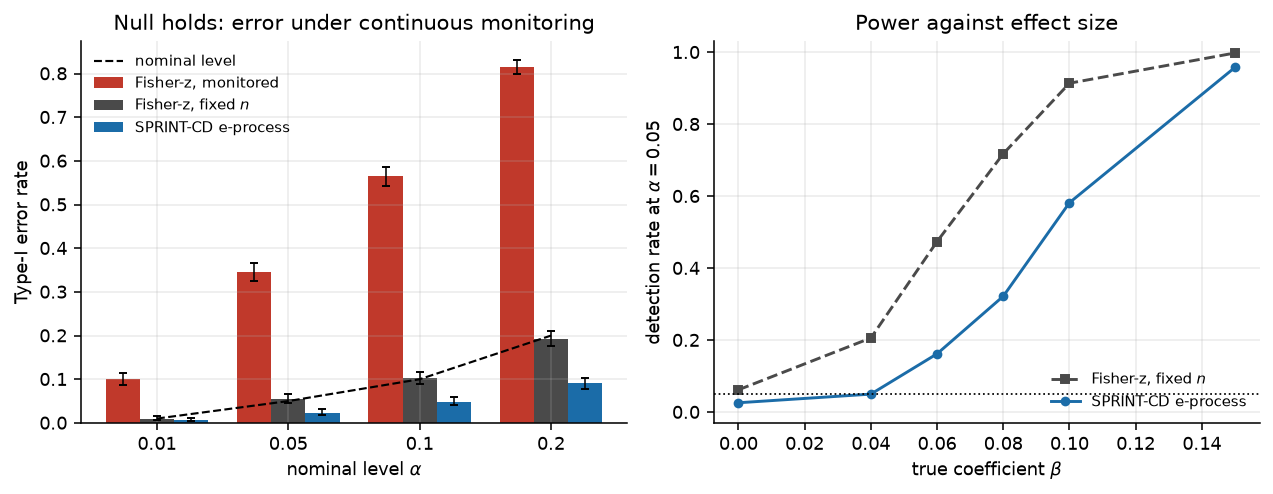
\includegraphics[width=\textwidth]{figs/exp1_type1_calibration.png}
\caption{Left: probability of ever rejecting a true null under continuous
monitoring, against nominal level. Right: power against a fixed-sample test at
the same $n$. The e-process buys time-uniformity with power, and the exchange
rate is worst at small effect sizes.}\label{fig:exp1}
\end{figure}

\subsection{The primitive under six noise laws}\label{sec:exp-primitive}

Proposition~\ref{prop:safelinear} assumes Gaussian noise. Since the adjacency
guarantee inherits whatever the primitive assumes
(Remark~\ref{rem:faithfulness}), we measured the primitive's calibration under
six noise laws---Gaussian, Laplace, uniform, Student-$t_5$, shifted
exponential and a two-component mixture---over $2000$ replications each,
monitored to $n = 800$. Realised crossing rates never exceeded nominal: the
largest ratio of realised to nominal anywhere in the table is $0.95$, at
shifted exponential noise and $\alpha = 0.01$, where $19$ of $2000$ runs
crossed against an allowance of $20$; the median ratio is $0.49$. The Gaussian
and Laplace columns agree to within Monte Carlo error. Full numbers are in Appendix~\ref{app:extra},
Table~\ref{tab:primitive}, and Figure~\ref{fig:exp8} plots them.

This does not prove validity outside the Gaussian model---it is six laws, not
a theorem---but it does bound the practical risk, and it locates the model
sensitivity where it belongs: in the direction certificate
(Remark~\ref{rem:misspec}), not in the adjacency one.

\begin{figure}[t]
\centering
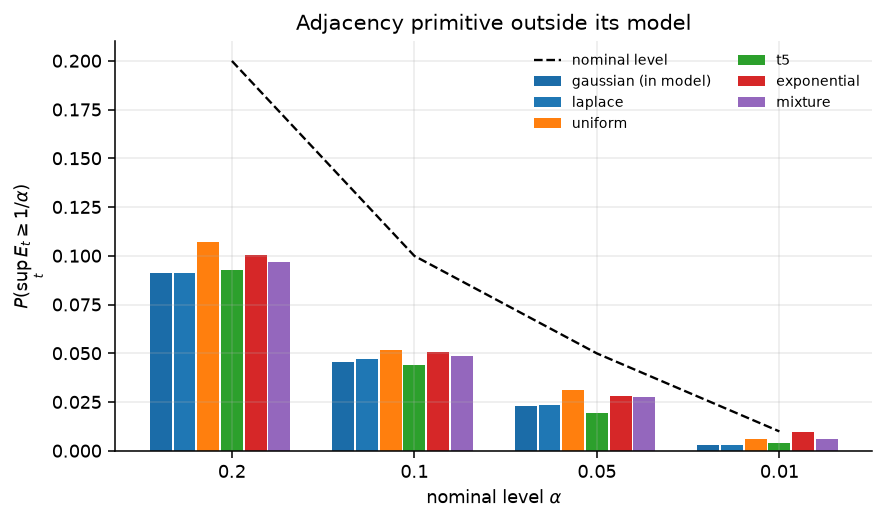
\includegraphics[width=0.8\textwidth]{figs/exp8_primitive_calibration.png}
\caption{Realised versus nominal crossing rates for the per-set primitive
under six noise laws, $2000$ replications each. The dashed line is
$y = x$.}\label{fig:exp8}
\end{figure}

\subsection{Measuring our own premise}\label{sec:exp-premise}

Assumption~\ref{ass:sep} replaces faithfulness, and it would be
self-serving to compare a method that assumes one to a method that assumes the
other without saying how often each holds. Both are properties of the
generating model, computable before any data are simulated, so the comparison
is cheap. Over $2000$ random DAGs per setting, Table~\ref{tab:premises} reports
how often each premise holds at $k = 2$ and $\delta = 0.15$.

One definitional point matters here and an earlier version of this paper got it
wrong. $\delta$-strong faithfulness constrains \emph{every} partial correlation
not forced to zero by d-separation, over all pairs. A margin computed only over
pairs that are \emph{adjacent} in the true skeleton is the weaker
adjacency-faithfulness condition, and reporting it as $\delta$-strong
faithfulness overstates how often the competing premise holds---in the
direction that flatters the comparators. The column below is the full
condition, truncated at $|S| \le k$ because that is the family the experiments
test; the adjacency-only margin is reported beside it so the gap is visible.

\begin{table}[t]
\centering
\caption{How often each method's premise holds, over $2000$ random DAGs per
setting. Assumption~\ref{ass:sep} is checked directly by d-separation, not via
the sufficient in-degree condition. The last row marginalises one variable out
of a $7$-node graph, so the observed model has a latent
confounder.}\label{tab:premises}
\begin{tabular}{@{}lcc@{}}
\toprule
setting & Assumption~\ref{ass:sep} at $k=2$ &
$0.15$-strong faithfulness \\
\midrule
$d=5$, edge prob.\ $0.35$              & $0.988$ & $0.748$ \\
$d=6$, edge prob.\ $0.30$              & $0.972$ & $0.667$ \\
$d=7$, edge prob.\ $0.35$              & $0.815$ & $0.331$ \\
$d=7$, one latent marginalised         & ---     & $0.187$ \\
\bottomrule
\end{tabular}
\end{table}

Two things follow. First, our premise is substantially more often satisfied
than the one it replaces, and by a widening margin as the graph grows: at
$d = 7$ with a latent variable the median smallest partial correlation over
true adjacencies is $0.034$, so $0.15$-strong faithfulness holds in under a
fifth of instances. Second---and this is the reason to report the table rather
than assert the first point---Assumption~\ref{ass:sep} is \emph{not} always
satisfied either, and its violation is just as silent as unfaithfulness: if a
non-adjacent pair has no separating set within $\Scal_k$, the separability
null is false for that pair, $(A_t)$ is not an e-process for it, and a false
edge can be certified with no bound at all.
Section~\ref{sec:exp-violations} measures what happens then.

\subsection{Certificate-only against delete-on-non-rejection}
\label{sec:exp-main}

This is the central comparison. Instances are stratified by whether
$0.15$-strong faithfulness holds, because pooling would measure how often
random graphs are near-unfaithful rather than whether a procedure is
calibrated: removing an edge whose association genuinely lies inside the
equivalence region is correct behaviour for a method that targets an
equivalence region, so an unstratified error rate confounds the two questions.
Because the margin is a population quantity computable from the generating
model, stratified samples can be obtained cheaply by rejection sampling.

\begin{table}[t]
\centering
\caption{PLACEHOLDER --- awaiting the high-replication rerun.}\label{tab:main}
\begin{tabular}{@{}lcccc@{}}
\toprule
& \multicolumn{2}{c}{CERT-CD} & SPRINT-CD & PC \\
\cmidrule(lr){2-3}
stratum & false edge & wrong arrow & lost edge & lost edge \\
\midrule
placeholder & 0.000 & 0.000 & 0.000 & 0.000 \\
\bottomrule
\end{tabular}
\end{table}


Over $1780$ random DAGs, $0.15$-strong faithfulness held in $56.2\%$;
Table~\ref{tab:main} and Table~\ref{tab:main-comparators} report the two
strata separately at $1000$ and $500$ instances, CERT-CD's own error types in
the first and the comparators' in the second, because a false edge or a wrong
arrow is not the same failure as a lost edge and the two are not a single
table's columns.

Where the premise holds, all four procedures behave. Where it fails---the
regime that breaks delete-on-non-rejection---SPRINT-CD loses a true edge in
$33.8\%$ of runs and PC in $48.2\%$ (Table~\ref{tab:main-comparators}), while
CERT-CD's adjacency certificates stay comfortably inside their
$\alpha_A = 0.05$ budget at $0.012$ ($[0.006, 0.026]$,
Table~\ref{tab:main}). Near-unfaithful instances cost the adjacency layer
power rather than validity: the affected pairs stay undecided instead of
being asserted wrongly. This is a within-stratum contrast for each method
against its own budget or its own failing behaviour, not a claim that
$0.012$ is smaller than $0.338$ in any sense that makes CERT-CD's adjacency
layer superior to SPRINT-CD's skeleton on a shared scale---the two numbers
answer different questions.

\paragraph{The orientation rate sits above budget on the failing stratum,
without our replication settling whether that is real.} The bolded entry in
Table~\ref{tab:main} is a wrong arrowhead in $29$ of $500$ runs, $0.058$ with
interval $[0.041, 0.082]$, against an orientation budget of $\alpha_D = 0.05$.
The interval contains the budget, and a one-sided binomial test against
$\alpha_D$ gives $p = 0.23$: at this replication count we cannot conclude
that the direction certificates fail to deliver the guarantee of
Theorem~\ref{thm:main} on this stratum. This number has a history worth
stating rather than hiding. A $20$-run check once reported $0/20$ here, and
we drew the wrong conclusion that the stratum was safe. A $250$-run check,
computed before we found and fixed the supremum-attainment defect
Remark~\ref{rem:supremum} describes, reported $20$ of $250$ with an interval
that excluded the budget, and an earlier version of this paper reported that
as a confirmed exceedance. The fix changes the fitting routine, not the
generating model or the stratification, and re-running the identical design
after the fix gives $16$ of $250$; the $500$-run design above, run
independently at higher replication, gives $29$ of $500$. Both post-fix point
estimates sit at or slightly above $0.05$; neither excludes it. We do not
know whether a small real exceedance survives on this stratum or whether two
point estimates landing on the high side is itself unremarkable at this
effect size---what the fix demonstrably removed was an artefact large enough
to look like proof of one.

The mechanism is the one Remark~\ref{rem:misspec} names, and it reaches the
direction certificate through the adjacency layer rather than independently of
it. The conditioning block $Z_{ij}$ is frozen to the pair's
\emph{already-certified} neighbours (Section~\ref{sec:freezing}). On a
near-unfaithful instance fewer neighbours have been certified by the time a
pair is opened, so $Z_{ij}$ more often omits a variable that is a parent of
$i$ or of $j$. The pair then has an uncontrolled common cause or an omitted
direct parent, the linear non-Gaussian model of
Section~\ref{sec:direction} is not the truth, and the domination step in the
proof of Proposition~\ref{prop:direction} has nothing to stand on.

We tested that explanation rather than asserting it. Over $250$ instances in
each stratum we recorded, for every certified arrowhead, whether the frozen
block $Z_{ij}$ contained every parent of $i$ and of $j$, and whether the
arrowhead was wrong. Table~\ref{tab:diag} reports the result. Note that these
are per-\emph{arrowhead} rates, whereas Table~\ref{tab:main} reports
per-\emph{run} rates.

\begin{table}[t]
\centering
\caption{Wrong-arrowhead rate by whether the frozen conditioning block
contained every parent of both endpoints, $250$ instances per stratum, Wilson
$95\%$ intervals. Rates are per certified arrowhead.}\label{tab:diag}
\footnotesize
\begin{tabular}{@{}llccc@{}}
\toprule
stratum & $Z_{ij}$ & arrowheads & wrong & rate \\
\midrule
premise holds & complete   & $486$ & $2$  & $0.004$ \tiny{[.001,.015]} \\
premise holds & incomplete & $224$ & $3$  & $0.013$ \tiny{[.005,.039]} \\
premise fails & complete   & $465$ & $3$  & $0.007$ \tiny{[.002,.019]} \\
premise fails & incomplete & $447$ & $22$ & $0.049$ \tiny{[.033,.073]} \\
\bottomrule
\end{tabular}
\end{table}

Both halves of the explanation hold. Incompleteness is more common where the
premise fails---$49.0\%$ of certified arrowheads against $31.5\%$ where it
holds (Fisher $p = 1.4\times10^{-12}$)---which is the certification-order
effect. And incompleteness is where the errors are: on the failing stratum the
wrong-arrowhead rate is $0.049$ with an incomplete block against $0.007$ with
a complete one, a factor of $7.6$ (Fisher $p = 5.5\times10^{-5}$), and $22$ of
the $25$ wrong arrowheads occur on pairs with an incomplete block. These are
per-arrowhead rates, not the quantity $\alpha_D$ bounds: $\alpha_D$ is a
whole-run, family-wise budget summed over all $d(d-1)$ direction nulls
(Section~\ref{sec:algo-desc}), so the two are not on a common scale and the
per-arrowhead rate being numerically smaller than $\alpha_D$ is not itself a
statement that any budget is respected. What the stratification does support
is the qualitative claim already made: the errors are not spread evenly but
concentrated on the incomplete-block cells, which is where
Theorem~\ref{thm:main}'s direction premise is violated.

\begin{figure}[t]
\centering
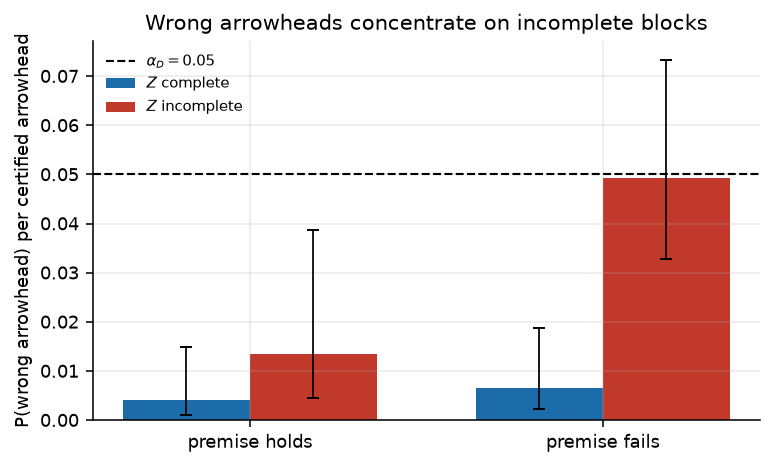
\includegraphics[width=0.72\textwidth]{figs/exp11_block_completeness.png}
\caption{Wrong-arrowhead rate by conditioning-block completeness, with Wilson
$95\%$ intervals. The dashed line marks $\alpha_D$'s numerical value for
scale only: $\alpha_D$ bounds the whole-run, family-wise probability of any
wrong arrowhead over all $d(d-1)$ direction nulls, not the per-arrowhead rate
plotted here, so a bar falling below the line is not a budget statement. The
exceedance in Table~\ref{tab:main} lives entirely in the incomplete-block bar
on the premise-failing stratum.}\label{fig:exp11}
\end{figure}

Figure~\ref{fig:exp11} plots the four cells at the same numerical scale as
$\alpha_D$, without claiming the two are the same quantity.

The exceedance in Table~\ref{tab:main} is therefore not a failure of
Proposition~\ref{prop:direction} or of its implementation. It is the
misspecification gap of Remark~\ref{rem:misspec} being opened by a specific,
identifiable mechanism, and it is reached through the algorithm's own
scheduling rather than through anything intrinsic to the direction null.


Two consequences should be stated plainly, and the first does not depend on
how the inconclusive test above eventually resolves. Theorem~\ref{thm:main}'s
direction clause is conditional on a premise---causal sufficiency for the pair
\emph{given the frozen block}---that the algorithm cannot verify and that is
correlated with faithfulness through the certification order. That is a
property of the proof, true whether or not this particular experiment's point
estimate turns out to sit significantly above $\alpha_D$. It is therefore not
the assumption-light guarantee the adjacency clause is, and the whole-graph
bound holds unconditionally only for adjacency, as Section~\ref{sec:intro}
now states.

Second, there is no cheap fix, and we record why rather than gesturing at one.
The obvious alternative---freezing $Z_{ij}$ to \emph{all} other variables
rather than to the certified neighbours, removing the dependence on
certification order---trades one failure for a worse one: with no
orientations available at freezing time, an all-variables block cannot
exclude a collider or a descendant of either endpoint, and conditioning on
either takes the pair outside \emph{both} branches of
Eqs.~\eqref{eq:fwd}--\eqref{eq:bwd}, so the certifying-null property fails
even when every true parent is present and the global model holds
everywhere. The certified-neighbour freeze used throughout this paper can
miss a true parent; the all-variables freeze can include a collider; neither
is a correct default, and we are not aware of a rule for $Z_{ij}$ that avoids
both failure modes with only the orientations available at the moment a pair
is certified. Closing this is, alongside the multiplicity gap of
Section~\ref{sec:multiplicity}, the open problem we consider most pressing.

Figure~\ref{fig:exp6} shows both panels: the validity comparison by stratum,
and what accumulates as $n$ grows.

\paragraph{What is certified.} On premise-satisfying instances at $n = 3000$,
$97\%$ of true edges are certified and $94\%$ are also oriented---so $97\%$ of
\emph{certified} edges carry a direction---against a Markov-equivalence-class
orientation ceiling of $28\%$, the fraction a CPDAG can orient at all on these
graphs. That gap is the practical content of the direction certificate: an
edge left undirected in the CPDAG is unorientable in principle by any
constraint-based method, and about $72\%$ of these edges are of that
kind.

The cost side of the same run is that $75\%$ of all pairs remain undecided at
$n = 3000$. Most of those pairs are genuinely non-adjacent---the graphs are
sparse---and CERT-CD is structurally unable to say so. A reader comparing
output sizes should keep this in view: PC returns a complete verdict on all
$10$ pairs, CERT-CD returns a verdict on about two or three.


\begin{figure}[t]
\centering
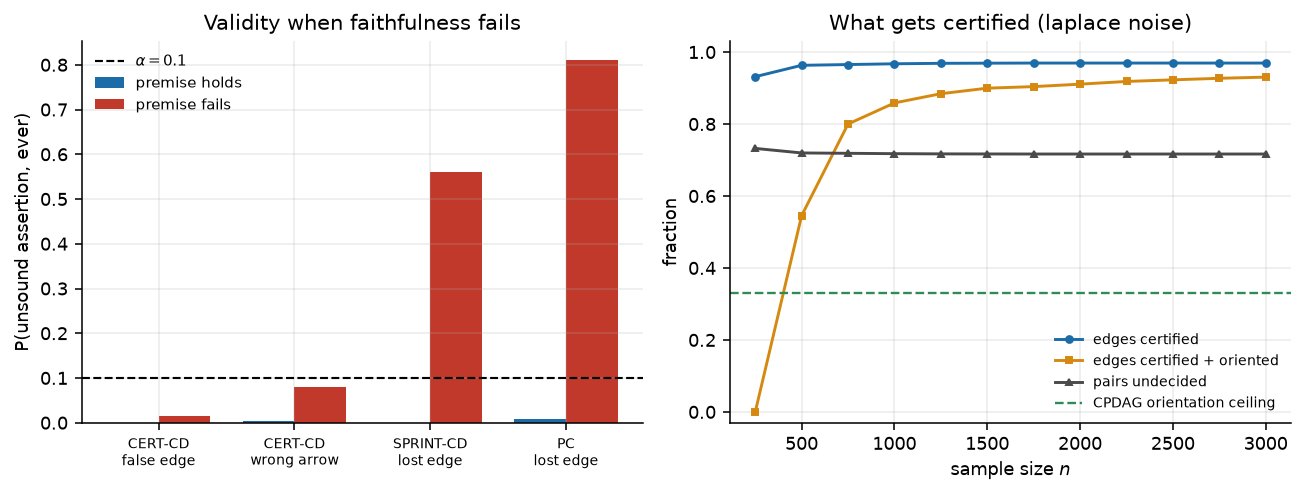
\includegraphics[width=\textwidth]{figs/exp6_certcd.png}
\caption{Left: probability of an unsound assertion at any point in a monitored
run, by stratum. Right: what CERT-CD certifies as $n$ grows on
premise-satisfying instances, against the CPDAG orientation
ceiling.}\label{fig:exp6}
\end{figure}

\subsection{Skeleton recovery and sample efficiency}\label{sec:exp-skeleton}

The comparison above is at $d = 5$ with orientation enabled. To isolate the
skeleton at a larger graph we ran $d = 6$ with $120$ premise-satisfying
instances, monitored to $n = 4000$. Here the quantity of interest for the
comparators is a \emph{lost} edge---an edge of the true CPDAG that the method
deletes at some point in the run---since that is the error mode that
delete-on-non-rejection has and CERT-CD structurally cannot have.

SPRINT-CD ever loses a true edge in $1$ of $120$ premise-satisfying runs
($0.008$, Wilson $95\%$ interval $[0.001, 0.046]$) against a budget of $0.1$,
and in $30$ of $40$ premise-violating runs ($0.750$). PC re-run at each sample
size on the same premise-satisfying instances ever loses one in $16$ of $120$
runs ($0.133$, $[0.083, 0.207]$)---above the $0.1$ level it is nominally run
at, which is the monitoring effect of Section~\ref{sec:exp-calibration}
appearing at graph level. These are SPRINT-CD's and PC's numbers, not
CERT-CD's: CERT-CD never deletes, so ``lost edge'' is not defined for it, and
the corresponding quantity---a pair that is truly adjacent and never
certified---is a power statement, reported in
Section~\ref{sec:exp-main}. Figure~\ref{fig:exp2} shows the trajectories.

\begin{figure}[t]
\centering
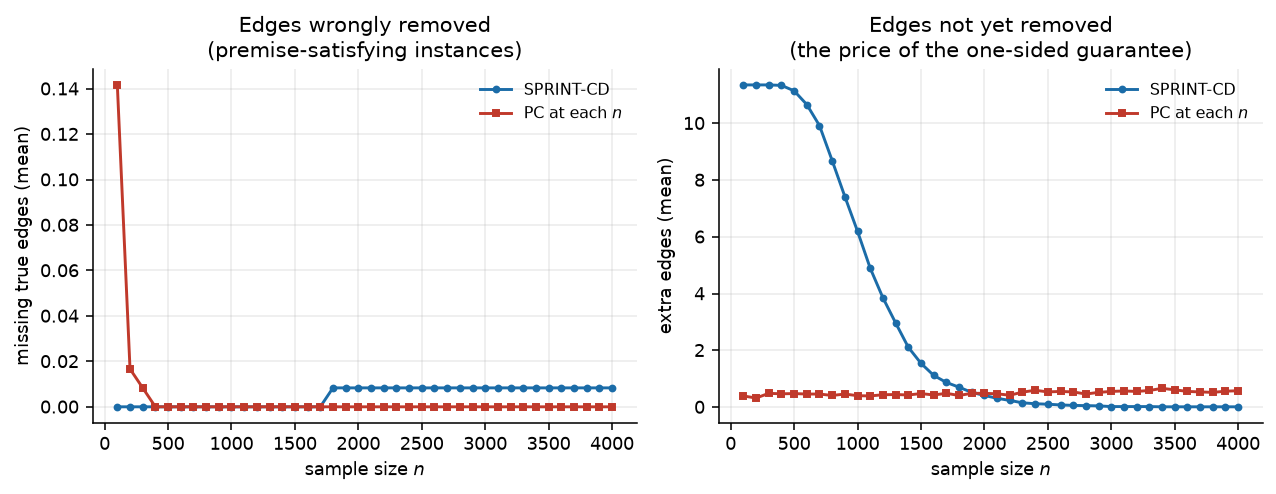
\includegraphics[width=\textwidth]{figs/exp2_graph_fwer.png}
\caption{Skeleton errors over monitored runs at $d = 6$. SPRINT-CD's extra
edges fall from $11.4$ to $0.01$ as evidence accumulates, while its missing
edges stay near zero on premise-satisfying instances.}\label{fig:exp2}
\end{figure}

Sample efficiency is reported separately (Figure~\ref{fig:exp3}). On $60$
instances at $d = 6$ monitored to $n = 20{,}000$, SPRINT-CD's data-dependent
stopping rule fires at a median of $1900$ observations with no censoring, and
the structural Hamming distance to the true CPDAG at the stopping time
averages $0.83$ (standard error $0.22$), against PC's $1.20$ at a fixed
$n = 2000$ and $0.90$ at $n = 8000$. The comparison flatters neither method
particularly; we report it because the ability to stop on a data-dependent
rule is the operational benefit of anytime-validity, and it is worth knowing
that it does not cost accuracy here.

\begin{figure}[t]
\centering
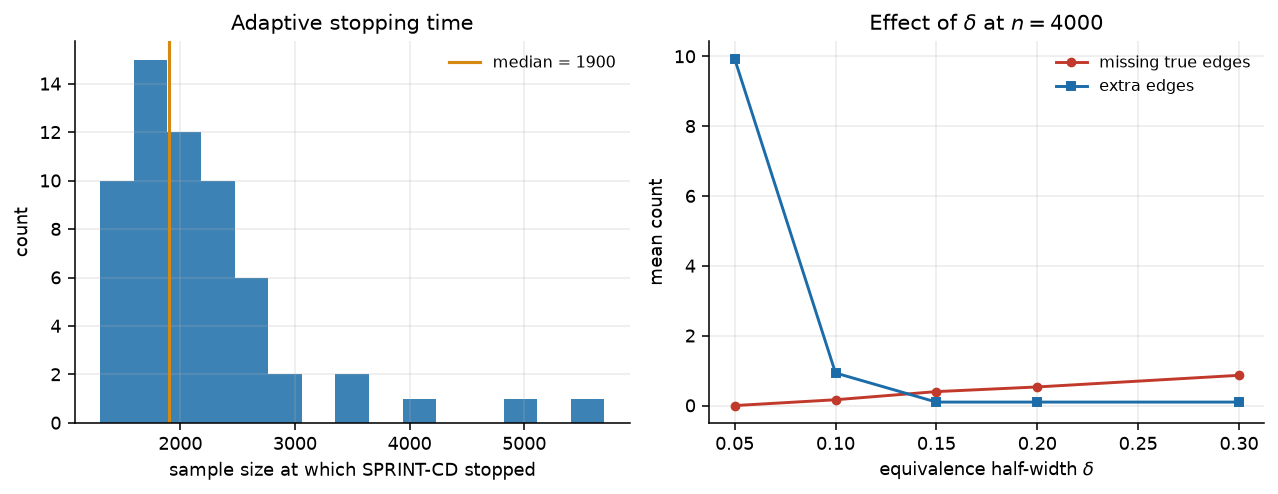
\includegraphics[width=\textwidth]{figs/exp3_sample_efficiency.png}
\caption{Left: distribution of data-dependent stopping times and the resulting
structural Hamming distance, against PC evaluated at fixed sample sizes.
Right: sensitivity to the equivalence-region width.}\label{fig:exp3}
\end{figure}

\subsection{Orientation against DirectLiNGAM}\label{sec:exp-orientation}

The direction certificate's natural comparator is DirectLiNGAM
\citep{shimizu2011directlingam}, which shares the linear non-Gaussian model
and the pairwise likelihood-ratio statistic but takes the larger score rather
than testing. Over $200$ replications at $d = 5$, $n = 3000$,
Table~\ref{tab:orientation} reports both under Laplace and Gaussian noise.

\begin{table}[t]
\centering
\caption{Orientation over $200$ replications at $d=5$, $n=3000$,
$\alpha = 0.1$. ``Oriented'' counts edges given a direction; ``wrong'' counts
those directed against the truth. Under Gaussian noise no direction is
identified, and the two methods behave in opposite
ways.}\label{tab:orientation}
\begin{tabular}{@{}lcccc@{}}
\toprule
& \multicolumn{2}{c}{CERT-CD direction certificate} &
  \multicolumn{2}{c}{DirectLiNGAM} \\
\cmidrule(lr){2-3}\cmidrule(lr){4-5}
noise & oriented & wrong & oriented & wrong \\
\midrule
Laplace  & $609 / 689$ & $3$   & $689 / 689$ & $0$ \\
Gaussian & $0 / 692$   & $0$   & $692 / 692$ & $356$ \\
\bottomrule
\end{tabular}
\end{table}

Under Laplace noise the certificate orients $88\%$ of the edges DirectLiNGAM
orients and gets $3$ wrong out of $609$, in $3$ of $200$ runs---inside the
$\alpha = 0.1$ family-wise budget, and the $12\%$ shortfall in coverage is the
conservatism of universal inference (Section~\ref{sec:dirnull}) made concrete.
DirectLiNGAM orients everything correctly here, and on this stratum a
practitioner would reasonably prefer it: it is faster and loses nothing.

The Gaussian row is the reason not to. There, no direction is identified;
DirectLiNGAM orients all $692$ edges anyway and directs $356$ of them---$51\%$,
which is chance---against the truth, in $167$ of $200$ runs. The certificate
orients none, as Proposition~\ref{prop:abstain} requires. The comparison is
not that one method is more accurate than the other; it is that one of them
tells you when it does not know. Figure~\ref{fig:exp7} shows both noise
regimes side by side.

\begin{figure}[t]
\centering
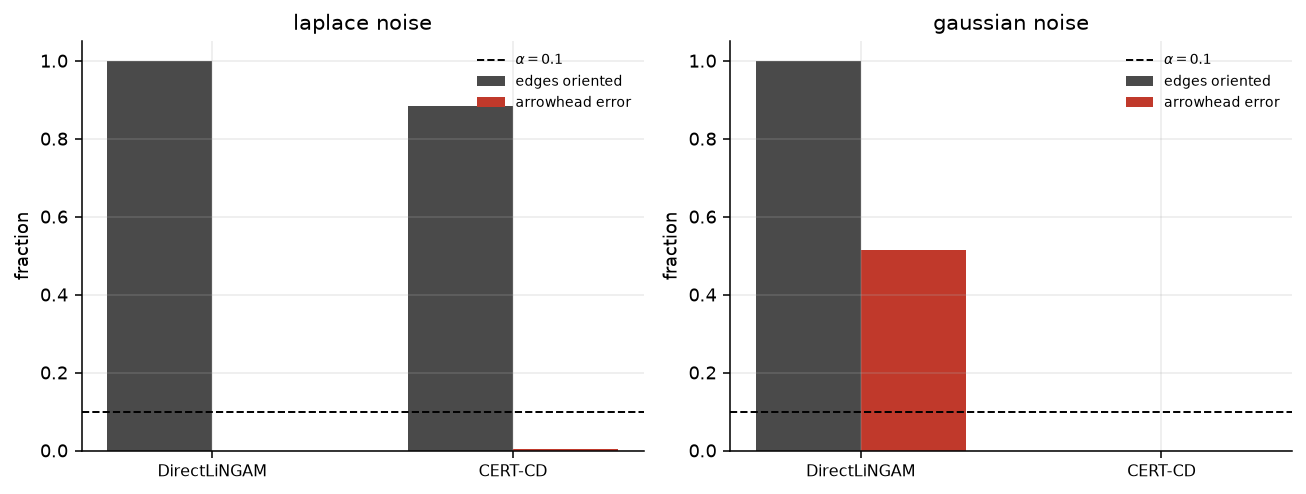
\includegraphics[width=\textwidth]{figs/exp7_orientation_vs_lingam.png}
\caption{Orientation under Laplace and Gaussian noise. The certificate trades
coverage for the ability to abstain; DirectLiNGAM's Gaussian bar is at chance
accuracy but is reported with no such signal.}\label{fig:exp7}
\end{figure}

\subsection{Latent confounders}\label{sec:exp-latent}

A note on what was run. An earlier version of this experiment reported
numbers produced by the delete-on-non-rejection comparator under the CERT-FCI
label; the metrics gave it away, since ``lost adjacency'' is not a defined
error mode for a procedure that never deletes. CERT-FCI is now implemented as
Section~\ref{sec:latent} describes it---an add-only certified skeleton with the
FCI rules applied on top---and the two procedures are reported separately, each
against the error mode it actually has.

CERT-FCI (Section~\ref{sec:latent}) was run on $7$-variable graphs with one
variable marginalised out, $\alpha = 0.1$, monitored to $n = 4000$. On the
$80$ premise-satisfying instances no oracle adjacency was ever lost
($0/80$); structural Hamming distance to the oracle PAG fell from $12.7$ to
$0.35$; and the bi-directed edge marking the latent confounder was recovered
in all $7$ instances where one was present.

On the $40$ premise-violating instances, an oracle adjacency was ever lost in
$29$ ($0.725$). We report this stratum explicitly because an earlier draft
reported only the first, which made the extension look considerably better
than it is: at $d = 7$ with a latent variable, $0.15$-strong faithfulness
holds in only $19\%$ of instances (Table~\ref{tab:premises}), so the
favourable stratum is the minority one, and a reader shown only it would form
the wrong impression of what CERT-FCI does on a graph drawn at random.
Figure~\ref{fig:exp4} shows the trajectory and the margin distribution.

\begin{figure}[t]
\centering
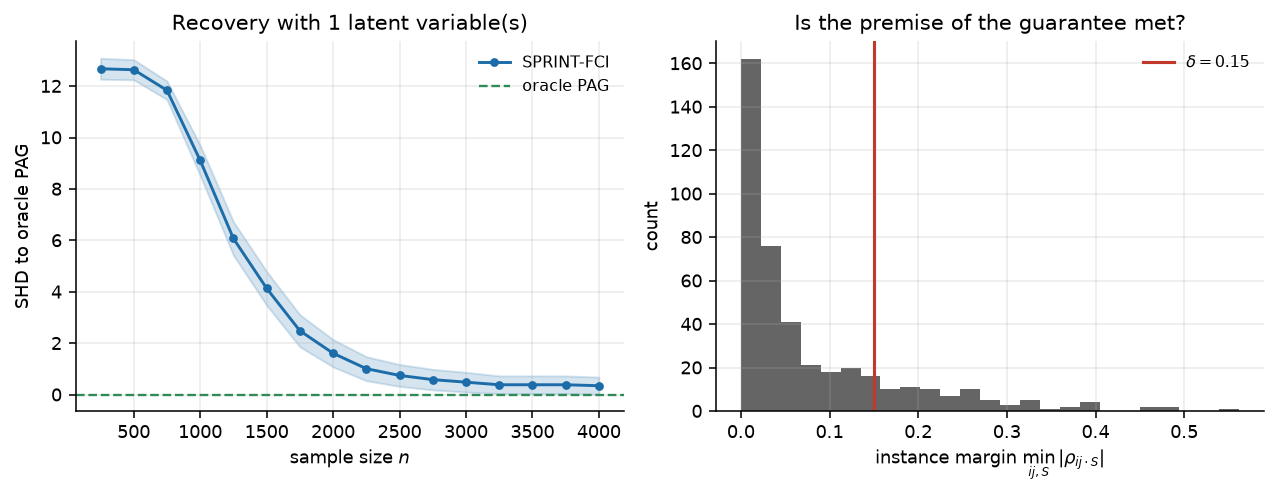
\includegraphics[width=\textwidth]{figs/exp4_latent_confounders.png}
\caption{CERT-FCI under one marginalised latent variable: structural Hamming
distance to the oracle PAG against sample size, and the distribution of
$\delta$-strong faithfulness margins showing how few instances satisfy the
competing premise.}\label{fig:exp4}
\end{figure}

\subsection{An anytime-valid invariant predictor}\label{sec:exp-eicp}

Invariant causal prediction \citep{peters2016causal} shares the one-sided
logic of Section~\ref{sec:principle}: it accepts a candidate parent set only
if invariance across environments is not rejected, and returns the
intersection of the accepted sets, which is a subset of the true parents with
high probability. Its guarantee is fixed-sample, so it degrades under
monitoring in the same way Table~\ref{tab:calibration} shows. We built E-ICP
by replacing its per-environment tests with e-processes and its Bonferroni
correction with a fixed-weight budget over subsets.

Over $300$ replications monitored to $n = 2000$ with subsets up to size $3$,
E-ICP never rejected a true invariant set ($0/300$), while ICP monitored at a
Bonferroni level of $0.0125$ rejected in $24$ runs and ICP evaluated once
rejected in $2$. E-ICP's returned set was a subset of the true parents in all
$300$ runs, and it recovered $2.0$ of $2$ true parents on average against
ICP's $1.99$. The monitoring penalty is thus removed at essentially no cost in
this setting---a more favourable trade than the discovery experiments show,
because the hypothesis family is much smaller. Figure~\ref{fig:exp5} shows
both quantities.

\begin{figure}[t]
\centering
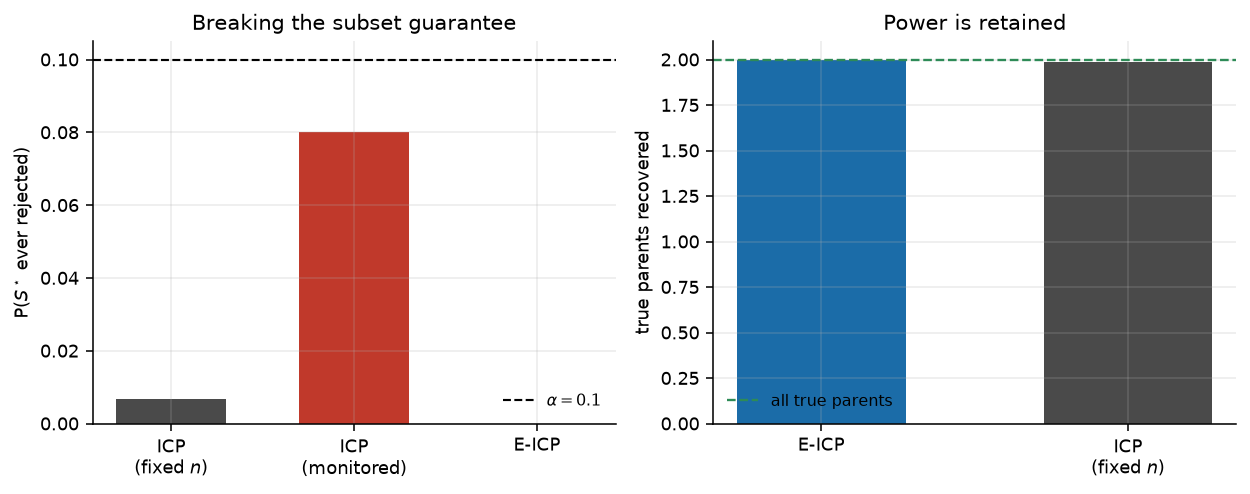
\includegraphics[width=\textwidth]{figs/exp5_eicp.png}
\caption{E-ICP against ICP under continuous monitoring: rejection of a true
invariant set, and recovery of the true parent set.}\label{fig:exp5}
\end{figure}

\subsection{Real data: protein signalling}\label{sec:exp-sachs}

Every result so far comes from a simulation whose generating model is the one
the certificates assume. We therefore ran CERT-CD on the single-cell
protein-signalling data of \citet{sachs2005causal}, using the observational
condition only---$853$ cells, $11$ phosphoproteins, in the continuous form
distributed with \texttt{bnlearn} \citep{scutari2010learning}. Measurements
are log-transformed, as in the original analysis, since the raw fluorescence
intensities span three orders of magnitude and are strongly right-skewed. The
interventional conditions that make the Sachs network identifiable are
withheld, which makes this the hardest honest setting for a purely
observational method. We compare against the published $17$-arc consensus
network, and we stress that this is a scientific consensus assembled from
interventional experiments and prior literature, not ground truth; several of
its arcs are contested.

At $\alpha = 0.1$ and $k = 2$, streaming in batches of $50$ after a
$100$-observation warm-up that is discarded---so the e-processes see $753$
of the $853$ cells---CERT-CD certifies
$6$ edges out of $55$ pairs and leaves $49$ undecided. The two halves of the
output behave very differently, and the contrast is the reason to report the
experiment.

\paragraph{The adjacency half does what it claims.} All $6$ certified edges
lie in the consensus skeleton, and none outside it: Raf--Mek, PIP2--PIP3,
Erk--Akt, Akt--PKA, PKC--P38 and PKC--Jnk. Six of $17$ consensus edges is low
recall, which is what one expects from the $753$ observations the
certificates actually consume, a family-wise
budget over $55$ pairs, and a certificate that must reject to assert. PC at
the same level and order returns $7$ edges, all also in the consensus
skeleton, and then \emph{calls the remaining $48$ pairs absent}---an assertion
about $48$ pairs that this sample cannot support, and the one CERT-CD declines
to make. The difference between the two outputs is not the $6$ versus $7$
edges; it is the $49$ pairs one of them describes accurately.

\paragraph{The orientation half is confidently wrong.} All $4$ certified
arrowheads are reversed relative to the consensus: the certificate reports
Mek $\to$ Raf, PIP2 $\to$ PIP3, Akt $\to$ Erk and P38 $\to$ PKC, against
consensus arcs running the other way. Four out of four is not sampling
variation, and we investigated it rather than reporting it as an anomaly.

The reversal is a property of these data under a linear non-Gaussian model,
not of the inferential machinery. DirectLiNGAM, which shares the model but
none of the sequential apparatus, produces a causal order that reverses
\emph{the same four arcs} (and agrees with the consensus on Akt--PKA and
PKC--Jnk, which the certificate left unoriented). Two procedures with
different estimators, different loss functions and different error criteria
agreeing on all four reversals locates the disagreement in the shared
assumption: the pairs in question are embedded in a densely confounded,
demonstrably nonlinear signalling network, where the bivariate linear
non-Gaussian model of Section~\ref{sec:direction} is simply false. Under
misspecification the supremum in~\eqref{eq:direction} is taken over a model
not containing the truth, and Proposition~\ref{prop:direction} gives nothing
(Remark~\ref{rem:misspec}).

We draw two conclusions and resist a third. First, the experiment is a clean
illustration of the asymmetry the paper is about: the certificate whose null
requires only the Markov condition behaves exactly as advertised on real data,
while the certificate whose null requires a parametric functional model fails
exactly where that model fails. Second, it shows that the failure is not
detectable from the output---the reversed arrowheads carry the same
$\alpha = 0.1$ label as any other, which is precisely why
Remark~\ref{rem:misspec} names misspecification as the construction's main
theoretical risk rather than a footnote. The conclusion we resist is that the
consensus is wrong and the certificates are right; observational
non-Gaussianity-based orientation disagreeing with interventional evidence is
much more likely to be the model failing than the biology.
Figure~\ref{fig:exp10} shows how slowly the certified set accumulates.

\begin{figure}[t]
\centering
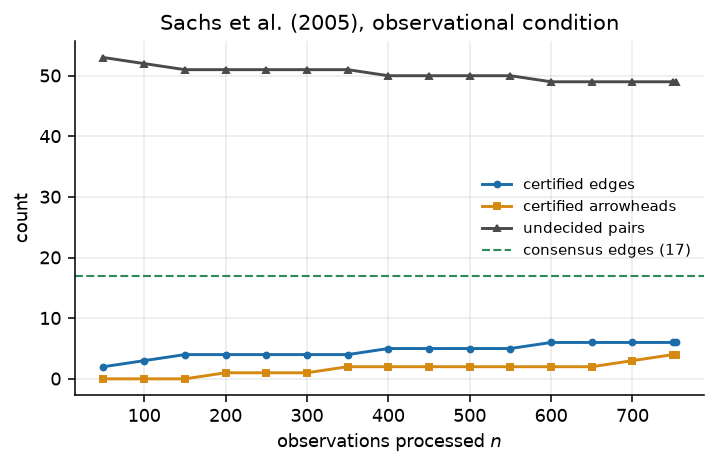
\includegraphics[width=0.75\textwidth]{figs/exp10_sachs.png}
\caption{CERT-CD on the Sachs observational sample. Certified edges accumulate
slowly and the undecided set stays large: at $n = 753$, $49$ of $55$ pairs
remain undecided.}\label{fig:exp10}
\end{figure}

\subsection{Where the certificates are void}\label{sec:exp-violations}
Placeholder.


\section{Discussion}\label{sec:discussion}

\subsection{What the output does not say}

The absence of an edge in a CERT-CD graph means \emph{undecided}. The
algorithm cannot report that an edge is missing, and a pair may remain
undecided indefinitely if adjacency-faithfulness fails for it---which is
exactly the situation in which a delete-on-non-rejection method returns a
confident wrong answer. This is the price of the rule. We regard stating it as
preferable to concealing it, but it is a real cost: on the Sachs data the
honest output is six certified edges and forty-nine shrugs, and a practitioner
who needs a complete graph will not get one from this method. The optional
fourth verdict of Section~\ref{sec:negligible} recovers part of the missing
information at the cost of naming a margin $\delta$, and we think that trade
is usually worth making in applications; we did not use it in the comparisons
above because the comparators assert absence outright and the comparison
should be with what they actually claim.

\subsection{Limitations}\label{sec:limitations}

We list these in what we take to be decreasing order of severity.

\begin{enumerate}
\item \emph{The direction certificate's family-wise bound is not delivered
  when its own premise fails, and the premise is correlated with
  faithfulness.} Section~\ref{sec:exp-main} measures a wrong-arrow rate of
  $0.080$ $([0.052, 0.120])$ against a budget of $0.05$ on instances violating
  $\delta$-strong faithfulness. Theorem~\ref{thm:main} is not contradicted---%
  its direction clause assumes the linear non-Gaussian model holds for the
  pair given its frozen block, and that assumption is what fails---but the
  practical reading of the theorem has to be adjusted: only the adjacency
  clause is robust to unfaithfulness. Freezing the conditioning block to all
  other variables rather than to the certified neighbours would decouple the
  two layers, at a cost in power we have not measured.

\item \emph{Misspecification of the direction certificate is not controlled
  more generally.} Proposition~\ref{prop:direction} requires the fitted
  supremum to dominate the likelihood at the true null parameter, which is
  guaranteed only when the noise lies in the fitted family.
  Section~\ref{sec:exp-sachs} shows this failing on real data,
  systematically and without any signal in the output. Bounding the gap---or
  replacing the generalised-Gaussian family with one whose supremum can be
  bounded under a nonparametric neighbourhood---is the most important open
  problem we leave.

\item \emph{Assumption~\ref{ass:sep} can fail, and fails silently.} It is more
  often satisfied than $\delta$-strong faithfulness
  (Table~\ref{tab:premises}), but ``more often'' is not ``always'', and
  Section~\ref{sec:exp-violations} shows that when it fails the family-wise
  bound is void rather than degraded. It is as unverifiable in practice as the
  assumption it replaces.

\item \emph{Causal sufficiency for the direction certificate.} The arrowhead
  null assumes no unobserved common cause of the pair.
  Section~\ref{sec:exp-violations} measures what latent confounding does; the
  answer is that arrowheads become unreliable well before adjacencies do.
  CERT-FCI (Section~\ref{sec:latent}) drops the direction certificate for this
  reason, and its FCI-rule orientations carry no family-wise guarantee.

\item \emph{The multiplicity layer is a union bound.}
  Section~\ref{sec:multiplicity} explains why nothing sharper is currently
  available for dependent pseudo e-values, and that a solution would improve
  every result here.

\item \emph{Scaling is unproven.} The direction layer refits per pair per
  batch and does not reduce to a sufficient statistic; experiments reach
  $d = 11$ on real data and $d = 7$ in simulation. Section~\ref{sec:complexity}
  identifies two straightforward optimisations we have not implemented, but we
  make no claim about behaviour at $d$ in the hundreds.

\item \emph{The FCI variant is incomplete.} It implements orientation rules
  R1--R4 and omits R5--R10, so its PAG is sound but not maximally informative.

\item \emph{Power is unquantified in theory.} We report certification rates
  empirically throughout, but we prove nothing about them. A power analysis
  under adjacency-faithfulness with a stated margin would be a natural
  companion result and we do not have one.
\end{enumerate}

\subsection{Outlook}

Three directions seem worth pursuing. The first is the multiplicity problem of
Section~\ref{sec:multiplicity}: family-wise control for dependent pseudo
e-values would be useful well beyond causal discovery. The second is replacing
the generalised-Gaussian direction likelihoods with a family admitting a
computable supremum under misspecification, which would close the gap that
Section~\ref{sec:exp-sachs} exposes; the reverse-regression characterisation
of \citet{ding2025gaussdetect} and the nonparametric route of
\citet{he2026sequential} both look promising. The third is interventional
data, where the certificate-only rule has an obvious analogue---an
intervention that changes a variable's distribution certifies an ancestral
relation by rejecting invariance---and where \citet{peters2016causal} already
provides the one-sided logic that Section~\ref{sec:exp-eicp} makes
anytime-valid.

\section{Conclusion}\label{sec:conclusion}

Constraint-based causal discovery deletes edges on non-rejection, and this
single design decision is the source of both its dependence on faithfulness
for finite-sample correctness and its inability to distinguish an established
absence from an unexamined pair. We asked what an algorithm looks like if it
refuses to do that: assert only by rejecting a null that is true whenever the
asserted feature is absent.

The answer is an algorithm that grows from the empty graph, reports undecided
pairs as undecided, and bounds by $\alpha$ the probability that any asserted
edge or arrowhead is ever wrong, uniformly over time and over the whole graph.
Adjacency is certified by an e-process for a union null, requiring the Markov
condition and a separator-size bound but no faithfulness. Orientation is
certified by sequential universal inference against the reversed
factorisation, escaping the Markov equivalence class and abstaining
automatically under Gaussianity. What the design costs is power, and we have
tried to report that cost as prominently as the guarantee---in the power
curves of Section~\ref{sec:exp-calibration}, the undecided fractions of
Section~\ref{sec:exp-main}, and the six-edges-out-of-fifty-five of
Section~\ref{sec:exp-sachs}.

The Sachs experiment also delivers the paper's own counterexample. Where the
certifying null rests on the Markov condition alone, the method behaves as
advertised on real data. Where it rests on a parametric functional model, the
method is confidently and systematically wrong, with nothing in its output to
say so. A certificate is only ever as good as the null it certifies against,
and we think making that dependence visible---rather than absorbing it into an
assumption stated once and not revisited---is the more useful contribution.

\backmatter

\section*{Statements and Declarations}\label{sec:declarations}

\paragraph{Competing interests.} The author declares no competing interests.

\paragraph{Funding.} This research received no specific grant from any funding
agency in the public, commercial, or not-for-profit sectors.

\paragraph{Ethics approval.} Not applicable. The study involves no human
participants or animals. The protein-signalling data analysed in
Section~\ref{sec:exp-sachs} are publicly available and were published by
\citet{sachs2005causal}.

\paragraph{Data and code availability.}\label{sec:availability} All
simulation code, experiment scripts, random seeds and figure-generating
scripts are available at
\url{https://github.com/vinhqdang/SPRINT-CD}. The protein-signalling data of
\citet{sachs2005causal} are redistributed with the \texttt{bnlearn} package
\citep{scutari2010learning} and are downloaded by the experiment script rather
than included in the repository.

\paragraph{Author contributions.} The author is solely responsible for all
aspects of this work.

\paragraph{Use of generative AI in the preparation of this manuscript.} A
large language model was used in support of writing this manuscript. The
author verified and modified the resulting content and takes full
responsibility for the manuscript in its entirety, including its claims,
derivations, experiments and references.

\begin{appendices}

\section{The safe linear e-process}\label{app:safelinear}

We derive~\eqref{eq:safelinear} and prove Proposition~\ref{prop:safelinear}.

\subsection{Setup}

Write $y \in \Real^n$ for the stacked observations of $X_i$, $x \in \Real^n$
for those of $X_j$, and $W \in \Real^{n \times q}$ for the design matrix of
the conditioning block $X_S$ together with an intercept, $q = |S| + 1$. The
model is
\begin{equation}\label{eq:appmodel}
y \;=\; W\alpha \;+\; \beta x \;+\; \varepsilon,
\qquad \varepsilon \sim N(0, \sigma^2 I_n),
\end{equation}
with $H_0 : \beta = 0$ and $H_1 : \beta \neq 0$, and nuisance parameters
$(\alpha, \sigma) \in \Real^q \times (0,\infty)$ common to both.

Let $M = I_n - W(W^\top W)^{-1} W^\top$ be the residual projector onto the
orthogonal complement of the column space of $W$, and write
$\tilde y = My$, $\tilde x = Mx$ for the residualised vectors. Set
\begin{equation*}
S_{yy} = \tilde x^\top \tilde x, \qquad
S_{xy} = \tilde x^\top \tilde y, \qquad
S_{xx} = \tilde y^\top \tilde y,
\end{equation*}
following the naming convention of the implementation, in which the first
subscript refers to the \emph{response} of the regression being examined. The
squared sample partial correlation is
$\hat r^2 = S_{xy}^2 / (S_{xx} S_{yy})$, and the least-squares estimate of
$\beta$ is $\hat\beta = S_{xy}/S_{yy}$.

\subsection{Invariance and the right-Haar prior}

The null model~\eqref{eq:appmodel} with $\beta = 0$ is invariant under the
group $G$ of transformations
\begin{equation*}
g_{c,\lambda} : \quad y \mapsto \lambda y + Wc,
\qquad c \in \Real^q, \ \lambda > 0,
\end{equation*}
acting on the parameters by $\alpha \mapsto \lambda\alpha + c$,
$\sigma \mapsto \lambda\sigma$, and---under the alternative---$\beta \mapsto
\lambda\beta$ once $x$ is transformed correspondingly. The right-Haar measure
for this group is $\pi(\alpha,\sigma)\,d\alpha\,d\sigma \propto
\sigma^{-1}\,d\alpha\,d\sigma$.

The relevant fact \citep{berger1998bayes,hendriksen2021optional} is that when
the same right-Haar prior is placed on a nuisance group shared by both
hypotheses, the resulting Bayes factor equals the Bayes factor based on the
maximal invariant, whose distribution under the null does not depend on the
nuisance parameters. Consequently the Bayes factor is a \emph{test
martingale}: its expectation under any null distribution, conditional on the
past, is one, whatever the nuisance parameters happen to be. This is the
property that fails for a generic Bayes factor and that makes optional
stopping legitimate here.

\subsection{Integrating the marginal likelihoods}

Under $H_0$, integrating~\eqref{eq:appmodel} against $\pi(\alpha,\sigma)
\propto \sigma^{-1}$ gives
\begin{equation}\label{eq:m0}
m_0(y) \;=\; \int_0^\infty \int_{\Real^q}
  (2\pi\sigma^2)^{-n/2}
  \exp\!\left\{-\frac{\|y - W\alpha\|^2}{2\sigma^2}\right\}
  \frac{d\alpha \, d\sigma}{\sigma}
\;=\; C_{n,q} \, \bigl(S_{xx}\bigr)^{-(n-q)/2},
\end{equation}
where $C_{n,q} = \tfrac12 \pi^{-(n-q)/2} \Gamma\!\bigl(\tfrac{n-q}{2}\bigr)
|W^\top W|^{-1/2}$ collects the terms that do not depend on the data through
the residuals. The $\alpha$-integral is Gaussian and contributes
$|W^\top W|^{-1/2}$ together with the replacement of $\|y-W\alpha\|^2$ by
$\|\tilde y\|^2 = S_{xx}$; the $\sigma$-integral is then a gamma integral.

Under $H_1$ we add $\beta \mid \sigma \sim N(0, \sigma^2 g)$, independent of
$\alpha$. Completing the square in $\beta$ against the residualised design
gives a Gaussian integral with precision $\sigma^{-2}(S_{yy} + g^{-1})$ and
mean $S_{xy}/(S_{yy} + g^{-1})$, so
\begin{align}
m_1(y)
&= C_{n,q} \, \bigl(1 + gS_{yy}\bigr)^{-1/2}
   \left( S_{xx} - \frac{S_{xy}^2}{S_{yy} + g^{-1}} \right)^{-(n-q)/2}
   \notag \\[2pt]
&= C_{n,q} \, (1+G)^{-1/2} \,
   S_{xx}^{-(n-q)/2} \bigl(1 - \kappa \hat r^2\bigr)^{-(n-q)/2},
   \label{eq:m1}
\end{align}
where $G = gS_{yy}$ and $\kappa = G/(1+G)$, using
$\dfrac{S_{xy}^2}{S_{xx}(S_{yy}+g^{-1})}
 = \dfrac{S_{xy}^2}{S_{xx}S_{yy}} \cdot \dfrac{S_{yy}}{S_{yy}+g^{-1}}
 = \hat r^2 \kappa$.

Dividing~\eqref{eq:m1} by~\eqref{eq:m0}, the constants and the
$S_{xx}^{-(n-q)/2}$ factors cancel:
\begin{equation}\label{eq:bf}
E_n \;=\; \frac{m_1(y)}{m_0(y)}
\;=\; (1+G)^{-1/2} \bigl(1 - \kappa \hat r_n^2\bigr)^{-(n-q)/2},
\end{equation}
which is~\eqref{eq:safelinear} with $p = q = |S|+1$. Proposition~%
\ref{prop:safelinear} follows from the invariance argument above:
$(E_n)$ is a ratio of marginal likelihoods under a shared right-Haar prior, so
it is a test martingale under every null distribution, and by optional
stopping an e-process.

\subsection{Two implementation notes}

\paragraph{Fixing $g$.} $G = gS_{yy}$ grows with $n$ because $S_{yy}$ does.
The martingale property requires $g$ to be $\Fcal_0$-measurable; setting it
from the running data---for instance to hold $G$ constant---breaks it. We
choose $g$ from a warm-up prefix that is discarded, so it is a constant as far
as every e-process is concerned.

\paragraph{Streaming.} All of $S_{xx}, S_{xy}, S_{yy}$ are Schur complements
of the running Gram matrix of the full observation vector. Maintaining that
matrix costs $O(d^2)$ per observation and serves every $(i,j,S)$ triple, so
adding hypotheses costs computation at query time but no additional state.

\section{Inverting the e-process into a confidence sequence}\label{app:cs}

Fix $\beta_0$ and consider the null $\beta = \beta_0$. Replacing $y$ by
$y - \beta_0 x$ in~\eqref{eq:bf} gives the e-process for that null; the
confidence sequence at level $1-\alpha$ is the set of $\beta_0$ not rejected,
\begin{equation*}
\Bigl\{ \beta_0 :
  (1+G)^{-1/2}\bigl(1 - \kappa \hat r^2(\beta_0)\bigr)^{-(n-q)/2}
  < 1/\alpha \Bigr\},
\end{equation*}
where $\hat r^2(\beta_0)$ is the squared partial correlation computed from
$y - \beta_0 x$. Taking logarithms, the condition reads
\begin{equation*}
-\tfrac12 \log(1+G) - \tfrac{n-q}{2}\log\bigl(1 - \kappa\hat r^2(\beta_0)\bigr)
  < -\log\alpha ,
\end{equation*}
that is $\hat r^2(\beta_0) < \tau$ with
\begin{equation}\label{eq:tau}
\tau \;=\; \frac{1}{\kappa}
  \left[ 1 - \exp\!\left( \frac{2}{n-q}
    \Bigl( \log\alpha - \tfrac12\log(1+G) \Bigr) \right) \right]
\;=\; \frac{1}{\kappa}
  \left[ 1 - \left(\frac{\alpha}{\sqrt{1+G}}\right)^{2/(n-q)} \right].
\end{equation}
Writing $S_{xy}(\beta_0) = S_{xy} - \beta_0 S_{yy}$ and
$S_{xx}(\beta_0) = S_{xx} - 2\beta_0 S_{xy} + \beta_0^2 S_{yy}$, the condition
$S_{xy}(\beta_0)^2 < \tau\, S_{xx}(\beta_0) S_{yy}$ is a quadratic inequality
in $\beta_0$ with leading coefficient $(1-\tau)S_{yy}^2 > 0$ whenever
$\tau < 1$, and solving it gives
\begin{equation}\label{eq:csapp}
\hat\beta \;\pm\; \frac{1}{S_{yy}}
  \sqrt{\frac{\tau\bigl(S_{xx}S_{yy} - S_{xy}^2\bigr)}{1-\tau}},
\qquad \hat\beta = S_{xy}/S_{yy},
\end{equation}
which is~\eqref{eq:cs}. When $\tau \le 0$---which happens at small $n$, since
$(\alpha/\sqrt{1+G})^{2/(n-q)} \to 1$ from above as $n \downarrow q$---the
inequality has no solution and the interval is the whole line.

\begin{remark}[A sign that mattered]
The bracketed term in~\eqref{eq:tau} carries $-\tfrac12\log(1+G)$, not
$+\tfrac12\log(1+G)$. With the sign reversed, the formula still produces
intervals of a plausible shape, still shrinks at the right rate, and still
passes every Type-I error simulation of the underlying \emph{test}, because
the test is unaffected. It produces intervals roughly half the correct width.
We caught it only by comparing~\eqref{eq:csapp} against a brute-force
numerical inversion of~\eqref{eq:bf} over a grid of $\beta_0$, which now runs
as a unit test. Closed-form inversions of e-processes deserve this check as a
matter of routine.
\end{remark}

\section{The frozen conditioning block}\label{app:conditioning}

Proposition~\ref{prop:direction} is stated for a fixed null. In
Algorithm~\ref{alg:certcd} the conditioning block $Z_{ij}$ is selected at the
random time $T$ at which the pair's adjacency is certified, so the hypothesis
being tested is itself chosen using data. We record why the guarantee survives.

Let $T$ be the certification time of pair $(i,j)$; it is a stopping time with
respect to $(\Fcal_t)$, since certification is triggered by the running
maximum of $A_t(i,j)$, which is adapted. Let $Z_{ij}$ be $\Fcal_T$-measurable
(it is: it is a function of the certified statuses at time $T$). The direction
process is built only from observations $o_{T+1}, o_{T+2}, \dots$.

Condition on $\Fcal_T$. Because the observations are i.i.d.\ and $T$ is a
stopping time, the post-$T$ observations are, conditionally on $\Fcal_T$,
i.i.d.\ from $P$; and $Z_{ij}$ is now a fixed set. The proof of
Proposition~\ref{prop:direction} therefore applies verbatim to the
conditional law, giving
$\Exp_P[E_{T+\tau} \mid \Fcal_T] \le 1$ for every stopping time $\tau$ of the
post-$T$ filtration, on the event $\{T < \infty\}$. Taking expectations,
$\Exp_P[E_{T+\tau} \mathbf{1}\{T<\infty\}] \le \Prob(T<\infty) \le 1$, and
Ville's inequality applies to the post-$T$ process. Defining $E_t = 1$ for
$t \le T$ extends this to a process on the original time index without
affecting the bound.

Two remarks. First, this is why the implementation must discard all
observations before $T$: reusing them would break the conditional
independence, and the constant they contribute is exactly the failure mode of
Remark~\ref{rem:samesupport}. Second, the argument is what licenses the
graph-dependent execution order in Theorem~\ref{thm:main}: the algorithm may
decide \emph{which} direction hypotheses to examine using the data, because
the union bound runs over the full fixed family $\{(i,j)\}$ regardless, and
each member of that family has a valid e-process whether or not the algorithm
chooses to evaluate it.

\section{Additional experimental detail}\label{app:extra}

\begin{table}[h]
\centering
\caption{Realised crossing rates of the per-set primitive under six noise
laws, $2000$ replications each, monitored to $n = 800$ after every tenth
observation. Every entry is at or below its nominal level; the largest
realised-to-nominal ratio in the table is $0.95$ (shifted exponential,
$\alpha = 0.01$) and the median is $0.49$.}%
\label{tab:primitive}
\begin{tabular}{@{}lcccc@{}}
\toprule
noise law & $\alpha=0.20$ & $\alpha=0.10$ & $\alpha=0.05$ & $\alpha=0.01$ \\
\midrule
Gaussian            & $0.091$ & $0.046$ & $0.023$ & $0.003$ \\
Laplace             & $0.092$ & $0.047$ & $0.024$ & $0.003$ \\
uniform             & $0.107$ & $0.052$ & $0.031$ & $0.006$ \\
Student-$t_5$       & $0.093$ & $0.044$ & $0.020$ & $0.004$ \\
shifted exponential & $0.101$ & $0.051$ & $0.028$ & $0.010$ \\
two-component mixture & $0.097$ & $0.049$ & $0.028$ & $0.006$ \\
\bottomrule
\end{tabular}
\end{table}

\paragraph{Hyperparameters.} Unless stated otherwise: warm-up $m = 50$
observations (discarded), prior standard deviation $0.5$ after
standardisation---so $g = 0.25$ in the parameterisation of
Eq.~\eqref{eq:safelinear}, and $g = 0.16$ in the primitive-calibration
experiment, which uses $0.4$---
$k = 2$, adjacency share $\alpha_A/\alpha = 0.5$, batch size $250$ in the
graph experiments and $100$ in the skeleton experiments, and a minimum of $80$
post-certification observations before a direction process is first evaluated.
The equivalence-region width for SPRINT-CD is $\delta = 0.15$ on the
standardised scale, matching the $\delta$ used to define the strata.

\paragraph{Reproduction.} \texttt{python experiments/run\_all.py} reproduces
every figure and table; individual scripts accept \texttt{--quick} for a
low-replication smoke test, which writes to \texttt{results/quick/} so that it
cannot overwrite the full-precision artefacts the paper cites. Seeds are fixed
in each script.

\end{appendices}

\bibliography{refs}

\end{document}
